% Stanford University PhD thesis style -- modifications to the report style
% This is unofficial so you should always double check against the
% Registrar's office rules
% See http://library.stanford.edu/research/bibliography-management/latex-and-bibtex
% 
% Example of use below
% See the suthesis-2e.sty file for documentation
%

\documentclass{report}
\usepackage{suthesis-2e}
\dept{Psychology}

% packages specific to this dissertation
\usepackage{graphicx}
\usepackage{amsmath}
\usepackage{gensymb}

% bibliography
% ref: http://tug.ctan.org/info/biblatex-cheatsheet/biblatex-cheatsheet.pdf
\usepackage[backend=bibtex,natbib=true,style=apa]{biblatex}
\renewcommand\nameyeardelim{, }
\addbibresource{library.bib}
\DeclareLanguageMapping{english}{american-apa}

\begin{document}
\title{Computational linking models of\\human selective visual attention}
\author{Daniel Birman}
\principaladviser{Justin L. Gardner}
\firstreader{Kalanit Grill-Spector}
\thirdreader{Tirin Moore}
\secondreader{Anthony Norcia}

\beforepreface
\prefacesection{Preface}

To sample the important parts of the visual world observers make saccades, moving the high-resolution and color-sensitive fovea to informative locations. Choosing to make a saccade requires sampling the periphery and identifying potentially important parts of the visual scene. This \emph{covert attention}, without eye movement, is essential to selecting information in an efficient manner. At an intuitive level, covert attention is a focusing on a feature or a location in the visual world and, in tandem, a suppression of other irrelevant features and locations. When operationalized into the laboratory, cueing an observer with covert attention can be shown to result in improved detection, smaller thresholds of discrimination, faster reaction times, and suppression of distractors. These changes are known to be in part the result of small tweaks to the representation of visual stimuli in sensory cortex, but are also the result of context-dependent selection occurring after sensory processing has gone to completion. How attention implements this balance of sensory change and selection is a central problem for the neuroscience of vision.

The first goal of this dissertation was to measure the strength of different forms of visual selection. If different ways of selecting from visual scenes (e.g. by color, or by location) result in different enhancements in performance, then they may be implemented in different ways in the brain. To test this, I developed an experimental paradigm in which an observer's perceptual sensitivity could be measured while selecting information in different ways. I showed that a small disadvantage to feature-based selection is the result of spatially overlapping distractors biasing responses. The consistent improvement in sensitivity observed across different forms of selection confirms that they may all be the result of a common form of selection. 

In the second and third parts of this dissertation I directly investigate the mechanism of feature-based selection. I first created a quantitative framework which characterizes how human visual cortex is sensitive to the properties of motion visibility. I then use this framework to build what we call a \emph{linking model}, a computational model which describes the steps from sensory representation to perceptual decision making. I then collected a large a dataset of human observers selecting visual information according to different visual features. I showed, using the framework and model, that our measurements are consistent with an implementation of selective visual attention that involves both enhancement (and suppression) of sensory representations as well as change in the downstream readout. 

Together, these results contribute to our understanding of human selective visual attention and demonstrate that selection is a process that involves the whole brain, not only sensory cortex. 

\prefacesection{Acknowledgments}
% This dissertation would not have been possible without the incredible patience of the (approximately) sixty volunteers who participated in my experiments. I am grateful for their willingness to see a ten-hour experiment as a challenging form of meditation and for the resolve of many of the participants to return over-and-over throughout my time at Stanford.



\afterpreface

\chapter[Introduction]{Selective visual attention}

\section{Visual attention}

We all know, more or less intuitively, what it is like to attend to something that we see. Hikers, for example, when on a dangerous trail may be particularly motivated to focus on the stability of their foot placements to avoid stepping on a loose rock, while ignoring the sights and sounds of the forests around them. The ease with which we can deploy attention hides a complex set of changes which occur inside the brain and which change our sensory perceptions.

In early attention research, observers used introspection to evaluate how their sensory experiences changed when they focused in various ways. These early researchers found that attention could change the conscious perception of a stimulus, making it more intense or clear \citep{Helmholtz1924-rl,James1981-cj,Kuelpe1902-qz,Titchener1908-bx}. These intuitions were not without merit, as spatial attention to some stimuli does appear to lead to a change in the appearance of a stimulus \citep{Carrasco2018-sb}. But without concepts to tackle the ideas of mechanisms and computation these authors never succeeded in making headway into how attention might be implemented in the human brain. 

Introspection yielded in the middle of the 20th century to more quantitative approaches in which attention, broadly defined, was operationalized into specific tasks. This allowed researchers to begin to make claims about the algorithm of attention. In particular, psychophysicists in the mid-20th century used reports about unattended stimuli to understand how information was selected. Perhaps the earliest example of this is a set of experiments in which observers were asked to echo speech from one ear at a time \citep{Cherry1953-as}. The transition from introspection to ‘objective’ measurement can be highlighted in the way these experiments were introduced, quoting from Cherry (1953): ``the `subject' under test (the listener) is regarded as a transducer whose responses are observed when various stimuli are applied, whereas his subjective impressions are taken to be of minor importance''. This approach was effective. The field made an abrupt move toward understanding sensory systems as processing units. Any given stimulus could be processed in a serial or parallel manner and processing might go to ‘completion’ or be halted at a certain point. Measuring the knowledge of a subject about an attended or ignored stimulus therefore assesses the extent of processing which has occurred for that stimulus. For example, for the echoing task described above, an observer might be asked whether they had retained knowledge about an un-echoed (and therefore, unattended) voice. If they could recall simple low-level features, e.g. that the speaker had a higher-pitched voice, then a researcher could conclude that parallel processing  of both streams had occurred up to pitch processing. They could then also conclude that processing of the ignored stimulus had then been halted, before the point of complete semantic understanding. Such results led researchers to begin to distinguish between stages of processing: an early parallel stage in which incoming sensory information is processed without immediate limits in capacity, and a second limited capacity serial stage from which complex decisions could be made.

Several early theories of attention focused on when selection occurs relative to the parallel and serial stages of processing. These theories fell out of the observations made above, that some features of auditory, as well as other sensory, stimuli are available for decision making regardless of the observers focus while other features must be attended to be available. To reconcile these facts researchers suggested a bottleneck and proposed that this was the mechanistic implementation of selective attention. The first such modern theory was Broadbent’s Filter theory \citep{Broadbent1958-ny}, which included an early bottleneck. In Filter theory visual information is processed in parallel until low-level features (location, intensity, frequency) are resolved. At this point, parallel processing gives way to a serial ‘complete’ processing of object identity, form, etc. The alternative theory, late selection, suggests that processing occurs up to semantics in an unconscious parallel manner \citep{Deutsch1963-ac}. An example best illustrates the distinctions in these theories. Again, if an observer is echoing one speaker while ignoring a second, a late selection account predicts that a substantial amount of information is nevertheless available about the ignored voice. This is because late selection predicts that a semantic-level processing of speech will occur regardless of sensory selection, leaving high-level information available to an observer. Evidence for this comes from experiments in which observers orient to highly salient, but also very high-level features, such as their own name, even when focused on other tasks \citep{Moray1959-fn}. This suggests that not also features are processed in identical ways. Selection theories were expanded upon, based on this suggestion that features might differ in their form of processing and not be consistently selected out in one step. Instead, it was suggested that features might be attenuated \citep{Treisman1960-qs} or that selection might be limited by variable capacity at different stages of processing \citep{Kahneman1973-af}.

Selective attention has been most heavily studied in the visual domain, in part because of the close relationship between selecting information in the world and orienting of the eyes. Spatial orienting can occur both in an overt movement of the eyes, but also covertly without eye movements. This covert attention accelerates responses \citep{Eriksen1972-qj} (Posner, Snyder, \& Davidson, 1980) and both improves detection performance and increases discrimination sensitivity \citep{Carrasco2011-xp}. Cues about important locations can both be imposed externally on an observer (Posner, 1980) or the result of internal guiding of attention toward the cued location. Covert attention can also be both spatial, related to eye movements, or featural \citep{Rossi1995-wa} as described below for search tasks. Because of this close relationship between selection (due to eye movements) and vision, researchers have focused in particular on the implementation of selective attention in the visual system. 

\section{Implementations of selective visual attention}

Selective attention is a balancing act for the brain, which must weigh the possibility of needing unattended information against the strength of sensory selection. In an early selection theory, information is being thrown out before complete processing -- which could be potentially disadvantageous if that stimulus later becomes important for behavior \citep{Mack1998-nq}. Late 20th century research on attention was well aware of this fact, and researchers showed that in different contexts sensory selection can be more or less complete at filtering out irrelevant information. In a few particularly dramatic demonstrations (Haines, 1991; Mack & Rock, 1998; Neisser, 1979; Simons & Chabris, 1999) observers can be shown to entirely lose access to otherwise highly salient information, but only when performing a task with significant cognitive load \citep{Lavie2005-aw,Lavie2004-ub,Rees1997-hd}. In vision, like in audition \citep{Moray1959-fn}, some visual information is processed no matter what, as scene gist can survive inattention, perceptually \citep{Li2002-ji} and as decodable information from measurements of BOLD signal in visual cortex \citep{Peelen2009-us}. These examples highlight the delicate balance that the brain must maintain: with limited resources how should the brain allocate these to efficiently sample the sensory world? Early research on the implementation of attention put this question to the side while first exploring the possible effects of attention on sensory processing. In apparent contradiction with the specific bottlenecks proposed by early and late selection theories, physiologists found that behavioral selection results in neural changes throughout the brain: in early visual cortex (where, presumably ‘parallel’ processing occurs), higher visual cortex, and in non-sensory regions. Reconciling these observations with the behavioral effects of selective attention has become a major goal of cognitive neuroscience. 

Modern neuroscience now deploys a multitude of neural recording techniques to understand how behavioral selection might be implemented by the brain. Both at a coarse scale in humans and at the level of individual neurons in primates and, very recently, rodents. In humans and non-human primates attention has been shown to alter the response gain of neurons in the visual system, including in the LGN  (O’Connor, Fukui, Pinsk, & Kastner, 2002), in V1 (Motter, 1993), V2 (Buffalo, Fries, Landman, Liang, & Desimone, 2010; Luck, Chelazzi, Hillyard, & Desimone, 1997; Motter, 1993), V3 (Liu, Larsson, & Carrasco, 2007; Pestilli, Carrasco, Heeger, & Gardner, 2011; Saenz, Buracas, & Boynton, 2002; Silver, Ress, & Heeger, 2007), V4 (Buffalo et al., 2010; Connor, Gallant, Preddie, & Van Essen, 1996; Luck et al., 1997; McAdams & Maunsell, 1999; Moran & Desimone, 1985; Motter, 1993; Reynolds, Pasternak, & Desimone, 2000; Spitzer, Desimone, & Moran, 1988), V3A (Serences & Boynton, 2007),  MT (Beauchamp, Cox, & DeYoe, 1997; O’Craven, Rosen, Kwong, Treisman, & Savoy, 1997; Saenz et al., 2002; Seidemann, Poirson, Wandell, & Newsome, 1999; Serences & Boynton, 2007; Treue & Martínez Trujillo, 1999; Treue & Maunsell, 1996) and MST (O’Craven et al., 1997; Treue & Maunsell, 1996), and in IT cortex (Chelazzi, Duncan, Miller, & Desimone, 1998; Moran & Desimone, 1985). Using BOLD imaging these changes can be observed simultaneously throughout almost all of early visual cortex (Liu et al., 2007; Pestilli et al., 2011; Saenz et al., 2002; Silver et al., 2007) and ventral temporal cortex (Baldauf & Desimone, 2014). Although the neurochemical mechanisms of these effects remain unclear, muscarinic acetylcholine receptors are known to play a key role (Herrero et al., 2008). Changes to sensory representations occur both for spatial attention tasks (Klein, Harvey, & Dumoulin, 2014; McAdams & Maunsell, 1999; Mitchell, Sundberg, & Reynolds, 2009; Pestilli et al., 2011; Womelsdorf, Anton-Erxleben, Pieper, & Treue, 2006) and feature-based attention tasks (Baldauf & Desimone, 2014; Harel, Kravitz, & Baker, 2014; Huk & Heeger, 2000; Jehee, Brady, & Tong, 2011; Saenz et al., 2002; Sàenz, Buraĉas, & Boynton, 2003; Serences & Boynton, 2007; Treue & Martínez Trujillo, 1999).

As measurements of physiology have become commonplace researchers have also confirmed that not all visual properties are processed in an equal manner. Behavioral results predicted this (F. F. Li et al., 2002; Moray, 1959) and one of the easiest operationalized tasks in which to observe this is during search (Wolfe, 1994). In a search task, an observer will be cued in advance to reveal the location of a particular item, e.g. by pointing to it, or to assess its presence, e.g. by pressing a button to indicate that it is present. The item will be hidden among a set of distractors whose properties determine the difficulty of the task. Such tasks are trivial when the target stimulus differs from the distractors along certain key dimensions: color, orientation, spatial frequency. Trivial, in this case, means that the processing required to solve the task occurs in parallel and the solution is found by the observer in “one step”, so to speak. This matches with experiments in the early visual system which show that neurons are characterized by their tuning to orientation, spatial frequency, and to particular regions of visual space \citep{Barlow1957-by,Hubel1962-pn}. The tiling of these neurons across retinotopic space results in visual field maps, of which there are more than a dozen identified in human visual cortex \citep{Wade2002-tt,Wandell2007-pr,Wandell2011-td}. In these simple search tasks, it appears that early visual cortex performs computations largely in parallel across these maps. Differences in the strength of signals across these maps, for each feature, can then result in ‘pop out’ of the relevant stimulus (Nothdurft, 1993; A. Treisman, 1985). 

Difficult search tasks involve conjunctions of stimulus properties (Egeth, Virzi, & Garbart, 1984) which require attention to be directed in a serial manner to each item (A. M. Treisman & Gelade, 1980). The results from search experiments match the findings of early physiology experiments (Hubel & Wiesel, 1959, 1968) which showed that the early visual cortex starts by processing in parallel the same simple features which ‘pop out’ during search. Sharp differences in these features drive bottom-up attention, or salience, in which features that differ from their neighbors can cause an observer to orient to them. In contrast to this parallel stage, higher areas in visual cortex process complex stimuli such as objects, but this processing does not appear to occur in parallel for multiple objects, instead objects trade off for representation according to the focus of attention (Desimone, 1998). Instead of the repetitive receptive field structure in early visual cortex these areas have large receptive fields and retinotopic bias according to experience, for example there is a foveal bias in areas selective for faces and a peripheral bias in areas that are selective for locations (Levy, Hasson, Avidan, Hendler, & Malach, 2001). Importantly, the physiological effects of selective attention are not isolated to any one of these areas. 

Our understanding of the neural implementation has advanced dramatically thanks to recordings of neuronal populations from animal models. But animal models have also held back research in important ways. In general it is not possible to probe an animals memory about unattended stimuli, rendering many classic psychophysics paradigms difficult to interpret. Whether the implementation of attention in a primate trained over months is similar to that in a human trained over the course of minutes is an unknown at the moment. Recently, mice have been shown to be able to exhibit selective attention (McBride, Lee, & Callaway, 2019; Wang & Krauzlis, 2018). This is promising for understanding the role of different brain areas in attentional selection, but also concerning. The mice in these studies exhibit a bias which resembles selective attention, but they also have high lapse rates compared to human observers. One explanation is that mice continue to explore the experiment space (Pisupati, Chartarifsky-Lynn, Khanal, & Churchland, 2019) whereas humans who learn from rules do not. Correctly taking these differences into account, perhaps by linking animal research directly to parallel human research, has a good chance of overcoming these issues. 

Despite the many results showing that sensory representations change during directed attention researchers have yet to converge on a consistent algorithm which implements selection. Instead, a number of competing theories exist for how sensory selection might proceed, including changes in sensitivity (Reynolds et al., 2000; Serences & Boynton, 2007; Snyder, Yu, & Smith, 2018; Treue & Martínez Trujillo, 1999), shifts in feature selectivity (Çukur, Nishimoto, Huth, & Gallant, 2013; David, Hayden, Mazer, & Gallant, 2008; Kastner, De Weerd, Desimone, & Ungerleider, 1998; Klein et al., 2014; Spitzer et al., 1988; Womelsdorf et al., 2006; Womelsdorf, Anton-Erxleben, & Treue, 2008), increases in baseline response (Buracas & Boynton, 2007; Chen & Seidemann, 2012; Fang, Boyaci, Kersten, & Murray, 2008; Kastner, Pinsk, De Weerd, Desimone, & Ungerleider, 1999; X. Li, Lu, Tjan, Dosher, & Chu, 2008), and changes in the structure of stimulus-driven and noise correlations (Cohen & Maunsell, 2009, 2011; Mitchell et al., 2009; Ruff & Cohen, 2016; Verhoef & Maunsell, 2017). All of these changes affect the information present in sensory cortex to different degrees. Depending on the overlap and correlation between stimulus representations enhancement to one stimulus may results in loss of information for another. In contrast with these theories, flexible readout which leaves stimulus representation unchanged (Birman & Gardner, n.d.) may be a useful alternative when behavior needs to remain adaptable. Deciphering the balance of sensory change against change in readout requires models which can quantify the extent to which neural changes result in behavioral changes. 

\subsection{Computational linking models}

Measurements of the neural effects of selective attention are not sufficient to understand its implementation, they must be linked correctly to behavior. To reconcile changes in cortical activity with behavior, cognitive neuroscientists can link measurements of neuronal activity and behavior using computational linking models. One assumption underlying much of cognitive neuroscience is that when we make a measurement of cortical activity, we are seeing the same signals that the brain uses the solve sensory decision making. This is only an assumption; it is possible that sensory decision making (and other forms of neural processing) are based on subsets of signals, or population codes, which remain harder to measure. To avoid making errors in inference it is important to make these hypotheses (or assumptions) about implementation explicit in a form which can be tested against other possible hypotheses. One way to do this is to build computational models which lay out the steps from sensory signal to sensory decision. We refer to these as “linking models”, as they link together perceptual measurements and cortical ones. 

Recent work has begun to explore computational models which link measures of behavior to neuronal recordings, i.e. building linking models (Barlow, 1972; Brindley, 1960; Cohen & Maunsell, 2010; Cook & Maunsell, 2002; Newsome, Britten, & Movshon, 1989; Pestilli et al., 2011). These experiments have shown that sensory responses are enhanced during directed attention while noise unrelated to the stimulus is altered and reduced (Ecker, Denfield, Bethge, & Tolias, 2016; Rabinowitz, Goris, Cohen, & Simoncelli, 2015; Snyder et al., 2018), which may be sufficient to cause neural activity to “align” to the dimension of readout (Ruff, Ni, & Cohen, 2018). In human research similar tasks have been shown to cause estimates of receptive fields to shift (Klein et al., 2014) which might be sufficient to enhance spatial sensitivity at attended locations (Klein, Paffen, Pas, & Dumoulin, 2016; Vo, Sprague, & Serences, 2017) consistent with a response gain occurring in earlier layers of the visual system (Baruch & Yeshurun, 2014; Miconi & VanRullen, 2016).
 
% In recent work, we have used computational linking models to show that change in sensory representation cannot be the sole implementation of attention during selective attention to motion visibility (Birman & Gardner, n.d., 2018). Using BOLD imaging we carefully measured how retinotopic visual cortex changed when observers were exposed to changes in the visibility of random dot motion patches. Using a perceptual discrimination task, we measured human perceptual sensitivity to these same stimulus properties. We then created a series of hypotheses about how sensory decision making might be solved in such a task and made our hypotheses explicit by instantiating each as a candidate linking model. For example, when asked to report about one stimulus feature such as contrast, but not about another such as the coherence, the brain might resort to enhancing and suppressing their respective sensory representations. Alternatively, the brain could leave sensory representations alone while changing downstream readouts. In these experiments, we found that models which had both a small amount of sensory change and a downstream readout best explained the data. Without the linking model, it is possible that we would have concluded that sensory changes alone implement such a context-dependent behavior, not knowing that they were quantitatively insufficient in our measurements.  

In a recent paper Pestilli et al. (Pestilli et al., 2011) found that a simple linking model of response gain during spatial attention was quantitatively insufficient to explain behavior. In that work, the authors found that a different form of readout was necessary to explain how the seemingly small changes in sensory representation could lead to large improvements in perceptual sensitivity. In non-human primates, linking models have been used to hypothesize about the possible roles of single neurons or populations in sensory decision making (Newsome et al., 1989). Similar results in humans have implicated early visual cortex as a source of information about contrast discrimination (Boynton, Demb, Glover, & Heeger, 1999). Finally, hypotheses about how sensory selection might alter the population code in cortex have been tested with linking models as well (Cohen & Maunsell, 2011). Although none of these examples involve causal manipulations (although they often depend on the results of such research) they nevertheless have considerable value to the field because they make explicit their assumptions about how sensory decision making proceeds.

Linking models have the additional advantage that they allow researchers to begin to speculate about why sensory selection might be implemented in different ways. Depending on where sensory information is represented selection may have to occur in different ways: scene gist, which survives inattention (F. F. Li et al., 2002; Peelen et al., 2009), may require very different kinds of selection to suppress compared to irrelevant spatial information (Pestilli et al., 2011). Task demands likely also change the form of selection, as well as the computational costs associated with different cortical implementations (Gardner, 2019). Changing sensory representations during selective attention may reflect a computationally efficient solution where the visual system is discarding, and therefore not fully processing, stimuli that are irrelevant to behavior. In contrast, flexible mechanisms which compute sensory decisions in a context-dependent manner (Mante, Sussillo, Shenoy, & Newsome, 2013) may require resources to represent and process stimuli that may not ultimately be behaviorally relevant. 

\section{Dissertation scope}

In this chapter, I have summarized literature relevant to our current understanding of selective visual attention. The goal of this dissertation is to test two of the aspects of sensory selection which remain poorly understood.

\subsection{Aim 1: Comparing spatial and feature-based attention}

Although we know that different visual features are processed in different ways, this does not necessarily mean that selection by these features requires different computational resources. It is also unclear whether selection by one feature, such as space, might be more efficient or strong than selection by a different feature such as color.

\textbf{In Chapter 2, I address this aim by building a psychophysics experiment with which I compare the strength of spatial and feature-based attention on a common metric.} I demonstrate in these experiments that the sensitivity (i.e. the variability in response error) is constant across different forms of selection, but that selection by feature is more likely to result in response bias from overlapped distractors. 

\subsection{Aim 2: Using linking models to compare implementations of selective visual attention}

The prevailing 



\chapter[Comparing spatial and feature-based attention]{Aim 1: Comparing spatial and feature-based attention on a shared perceptual metric}

\section{Introduction}

The demands of everyday life require us to flexibly shift our attention between many different aspects of the visual world. When researchers operationalize these behaviors they often turn to tasks in which an observer must select information from the visual scene either from a spatial location or a particular feature dimension. This distinction has led to categorizing covert visual attention into two types: spatial attention, when task demands require selecting information at a specific location and not others, and feature-based attention, where task demands require selecting some features (e.g. colors, spatial frequencies, motion directions, etc) but not others. This categorization could reflect a real physiological difference in how spatial and feature-based attention are implemented by the brain. An alternative though is that space is not privileged over other features in visual cortex, and that instead selection of information is a generic computation.

To relate different forms of selection we designed a set of experiments in which spatial and feature selection could be measured on the same perceptual metric. In one experiment this metric was the recall of a stimulus from working memory, and in a second a comparison of two perceptually similar stimuli. In both cases we cued observers to select two stimuli out of a set of four using either the stimulus features or spatial locations. We then model each task to estimate the underlying perceptual sensitivity in each selection condition. Our results suggest that selection is generic: perceptual sensitivity does not change according to the selection process. But, the likelihood of mistaking one stimulus for another is more likely when two stimuli are overlapping in space.


**PAge 98 in Pashler:
Search for a T or a green element, reporting presence and location in a N-AFC task. When detected the location can be reported, and if not correct then the probability is 1/N distributed. 
See Watson and Robson 1981
Graham 1989
See also Snyder 1972, reporting letter selected by color, more likely to make errors of spatial neighbors than far away neighbors. How to refute that if space = feature? See Nissen 1985 as well.
Tsal Lavie 1988 - 3 of each color letter, report one red + more, more likely to be neighbors than to be the same color. But is this just convenience because color vs. letter is at different levels? Same with Snyder, etc? Color vs. direction vs. space seems more reasonable test?


\section{Methods}

\subsection{Observers}
In total X observers were subjects for the experiments. All observers except one (who was an author) were naive to the intent of the experiments. X observers were excluded during the initial training sessions due to an inability to maintain appropriate fixation (see eye-tracking below). Procedures were approved in advance by the Stanford Institutional Review Board on human participants research and all observers gave prior written informed consent before they participated in the experiment. When necessary, observers wore corrective lenses to correct their vision to normal.

\subsection{Hardware setup for stimulus and task control}

Visual stimuli were generated using MATLAB (The Mathworks, Inc.) and MGL (Gardner et al., 2018). Stimuli were displayed on a 22.5 inch VIEWPixx LCD display (resolution of 1900x1200, refresh-rate of 120 Hz) and responses collected via keyboard. Output luminance and spectral luminance distributions were measured for the LCD display with a PR650 spectrometer (Photo Research, Inc.). The gamma table for each display was dynamically adjusted at the beginning of each trial to linearize the luminance display such that the full resolution of the 8-bit table could be used to display the maximum contrast needed. The luminance spectra were used to compute a transformation matrix from the L*a*b* color space [cite] to the RGB output of the screen, such that the a* and b* dimensions could be separately manipulated without changing the luminance (L*). Other sources of light were minimized during behavior.

\subsection{Eye tracking}

Eye-tracking was performed using an infrared video-based eye-tracker at 500 Hz (Eyelink 1000; SR Research). Calibration was performed throughout each session to maintain a validation accuracy of less than 1 degree average offset from expected using a thirteen-point calibration procedure. Trials were initiated by fixating the central cross for 300 ms and canceled on-line when an observer’s eye position moved more than 1.5 degree away from the center of the fixation cross for more than 300 ms. During training and before data collection. observers were excluded from further participation if we were unable to calibrate the eye tracker to an error of less than 1 degree of visual angle or if their canceled trial rate did not drop to near zero.

\subsection{Experimental design}

\subsubsection{Estimation task}

Stimuli consisted of two pairs of dot patches, to the left and right of a central fixation cross (0.5 x 0.5 deg). The dot patches were circular regions centered 7 degrees eccentric with a diameter of 10 degrees, thus covering from 2 degrees to 12 degrees along the horizontal axis. Each patch was filled with two sets of moving dots (X dots / deg^2, per set, Y deg diameter). Dots within a patch were given an identical color (equal luminance, with a* and b* varying) and moved in the same direction at X degs / sec. Dots were “alive” for Y secs before vanishing and reappearing immediately at a new random location.

On each trial in the estimation task observers were asked to report about either the color or motion direction for a single dot patch. Before each block of X trials observers were told which feature would be reported with either the phrase “report color” or “report direction” appearing on the screen. Key to the task was that although observers ultimately reported about only one dot patch they could be cued to remember just that patch, or multiple patches. 

\subsubsection{Comparison task}

The stimulus for the comparison task was identical to the estimation task, but the task differed. In this task observers were asked to report which of two paired stimuli were more similar in color or motion direction. The pairs could be defined by location (i.e. the two dot patches on the right vs. the two on the left) or by feature (e.g. the upward-moving patches on the left and right vs. the downward-moving patches on the left and right). We used a reaction time task and allowed observers to respond immediately. 

\section{Results}
\section{Discussion}

\chapter[A framework for motion visibility]{Aim 2: A quantitative framework for motion visibility in human cortex}
\section{Introduction}
Much of the neural basis of perception has been revealed by manipulations that control the visibility of motion stimuli. For example, global motion direction of random-dot stimuli is made less visible by decreasing motion coherence, i.e., the percentage of dots moving in the same direction. At lower visibility levels, small changes in cortical signals manifest in measurable behavioral effects, thus documenting direct links between cortical physiology and perception \citep{Britten1992-xy,Newsome1989-fr} and uncovering neural signals supporting evidence accumulation \citep{Huk2005-xg,Katz2016-xc,Roitman2002-mw,Shadlen1996-pr,Shadlen2001-uu}. Making stimuli brief also renders them less visible, aiding, for example, the study of information integration across eye movements \citep{Melcher2003-vw}. Increasing image contrast, the average difference between bright and dark \citep{Bex2002-it}, makes stimuli more visible and cortical responses monotonically larger allowing links to be made between cortical response and perception \citep{Boynton1999-jd,Ress2000-pa,Ress2003-lt}, disambiguating mechanisms for spatial attention \citep{Carrasco2000-es,Hara2014-tm,Hara2014-mv,Pestilli2011-gi}, uncovering neural correlates of conscious perception \citep{Lumer1998-qs,Wunderlich2005-ff}, and revealing the effects of putative priors \citep{Stocker2006-rk,Vintch2014-zu}. While each of these manipulations has been used extensively in the human perceptual literature, they can have greatly different effects on human neural response. Given the central importance of motion visibility, a quantitative model of response across human visual cortex is required to provide a framework for interpreting and building upon these various findings.

Such a population response model must quantitatively account for the shape of the relationship between motion visibility and cortical response. The response function for contrast has been characterized as a sigmoidal function for measurements in single units \citep{Albrecht1982-rq,Sclar1990-lk} and populations \citep{Avidan2002-jg,Boynton1996-ff,Boynton1999-jd,Gardner2005-pg,Logothetis2001-kk,Olman2004-dd} (Tootell and Taylor 1995; Tootell et al. 1998). Increasing motion coherence typically results in linear increases in response \citep{Aspell2005-tc,Britten1993-oh,Handel2007-xk,Rees2000-ul} (Simoncelli and Heeger 1998) although this may depend on the exact stimulus parameters \citep{Ajina2015-xm}.

A population response model must also quantify the variable sensitivity to visibility parameters across cortical areas. The earliest cortical areas have a larger dynamic range for contrast compared with later areas which are more invariant \citep{Avidan2002-jg,Cheng1994-ic,Rolls1986-wr,Sclar1990-lk}. Less is known about motion coherence sensitivity except that the neural response to coherent compared with incoherent motion or blank evokes a large response in the human middle temporal area (hMT+, referred to as MT) with some sensitivity reported in earlier visual cortical areas (Ajina et al. 2015; Costagli et al. 2014; Dupont et al. 1994; Heeger et al. 1999; Tootell et al. 1995; Watson et al. 1993; Zeki et al. 1991) and parietal and ventral regions (Braddick et al. 2001).

Finally this model must account for stimulus duration effects. Hemodynamic responses to visual stimuli are approximately temporally linear except when durations \citep{Boynton1996-ff,Boynton2012-xy} or inter-stimulus intervals \citep{Huettel2000-ji} are brief. The divergence from linearity may differ across cortical areas \citep{Birn2001-tp} and motion-sensitive regions may be most sensitive to transient changes \citep{Stigliani2017-oe}.

Here we measured blood-oxygen-level dependent (BOLD) \citep{Ogawa1990-er} response in human observers to a large range of contrast, coherence and duration of motion stimuli, and built a quantitative model linking these visibility properties with physiological response in retinotopically defined visual areas. Sensitivity to these parameters varied significantly across areas, although all were sensitivity to both contrast and coherence without interaction. While perceptual experiments have often used different means of affecting visibility interchangeably our results provide a reference model that underscores the differences in response to each manipulation of visibility across cortical areas, thus providing a quantifiable way to interpret experiments that link cortical response to perception.

\section{Methods}
\textit{Observers}

In total, 11 observers (8 female, 3 male; mean age 26 y; age range 19–36 y) were subjects for the experiments. All observers except one (who was an author) were naive to the intent of the experiments. Observers were scanned three times, in 2 two-hour sessions of the experiment and a one hour retinotopy session. Procedures were approved in advance by the Stanford Institutional Review Board on human participants research and all observers gave prior written informed consent before they participated in the experiment. When necessary, observers wore corrective lenses to correct their vision to normal.

\noindent
\textit{Hardware setup for stimulus and task control}

Visual stimuli were generated using MATLAB (The MathWorks) and MGL (Gardner et al. 2018b) (http://gru.stanford.edu/mgl). Stimuli were backprojected via an Eiki LC-WUL100L projector (resolution of 1,900×1,200, refresh rate of 100 Hz) onto an acrylic sheet mounted inside the scanner bore near the head coil. Visual stimuli were viewed through a mirror mounted on the head coil and responses were collected via an MRI-compatible button box. Output luminance was measured with a PR650 spectrometer (Photo Research) and a neutral density filter used to set the average screen luminance to 300 cd/m2. The gamma table was then dynamically adjusted at the beginning of each trial to linearize the luminance display such that the full 10-bit output resolution of the gamma table could be used to display the maximum contrast needed. Other sources of light were minimized during scanning.

\noindent
\textit{Eye tracking}

Prior to the experiment subjects were extensively trained on a behavioral task requiring precise fixation. Eye tracking was performed using an infrared video-based eye-tracker at 500 Hz (Eyelink 1000; SR Research). Calibration was performed throughout each session to maintain a validation accuracy of less than 1° average offset from expected using either a 10-point or 13-point calibration procedure. Trials were canceled online when observer’s eyes moved more than 1° away from the fixation cross for more than 300 ms. After training, canceled trials consisted of fewer than 0.1\% of all trials. Due to technical limitations eye tracking was not performed inside the scanner.

\noindent
\textit{Experimental design}

Motion stimuli consisted of two patches of moving dots and a central cross (1 × 1°) on which observers maintained fixation. The dot patches were rectangular regions extending from 3.5 to 12° horizontal and −7 to 7° vertical. Each patch was filled with 21 dots/\degree$^2$, 50\% brighter and 50\% darker than the gray background (300 cd/m2). Both patches maintained a constant baseline in between trials of 25\% contrast and incoherent motion. During a trial, the patches increased in either or both contrast and coherence. To minimize involuntary eye movements, the coherent dot motion direction was randomized to be horizontally inward or outward from fixation on each trial, such that each patch moved in opposite direction. All dots moved at 6\degree /s updated on each video frame. Motion strength was adjusted by changing motion coherence; that is, the percentage of dots that moved in a common direction with all other dots moving in random directions. Dots were randomly assigned on each video frame to be moving in the coherent or random directions.

We measured the cortical response to a wide range of brief increments of stimulus contrast and coherence of variable duration while observers performed an independent and asynchronous task at fixation (Fig. \ref{fig:c1f1}). Each scan began with a 30-s baseline period (25\% contrast, 0\% coherence) to allow visual cortex to adapt. Each trial consisted of a brief increment in either or both the contrast and motion coherence of the dot patches. The dot patches then returned to baseline (25\% contrast, 0\% coherence) for an inter---trial interval of 2 to 11 s (mean 6.5 s) randomly sampled from an exponential distribution. The next trial then began synchronized to the next volume acquisition of the magnet. Stimulus increments were chosen to be +0, +25, +50, or +75\% above the baseline 25\% contrast and +0, +25, +50, +75, or +100\% above the baseline 0\% coherence and lasted for 250, 500, 1,000, 2,000, 2,500 or 4,000 ms (or as close to these durations as the display frame refresh would allow). We presented trials in two sets; a “complete cross set” in which all combinations of contrast and coherence changes at 2,500 ms duration were presented (4 contrasts×5 coherences = 20 conditions) and a “duration set” in which a subset of the contrast and coherence combinations (+25 or +75 contrast and +25 or +100 coherence) were presented for variable stimulus durations (4 contrast and coherence combinations×5 stimulus durations = 20 conditions). Thus, across the complete cross and duration sets, there was a total of 40 conditions (20 each in the complete cross and duration sets). For each condition we acquired a minimum of 20 repeated presentations throughout the scan sessions of each observer, resulting in a minimum of 800 trials total. The two trial sets were presented in separate scans interleaved within sessions. Condition order within each scan, for both trial sets, was randomized independently for the stimulus on the left and right such that in every block of 40 trials all conditions were presented in both dot patches.

While these stimuli were being presented for the passive viewing condition, the observer was required to perform a luminance decrement task on the fixation cross. The fixation cross decremented twice in luminance for 400 ms, separated by an 800-ms interstimulus interval and the observer reported with a button press which decrement interval appeared darker (see Gardner et al. 2008 for details). Decrement amplitude was adjusted according to a staircase procedure to maintain ~82% correct.

\noindent
\textit{MRI acquisition and preprocessing}

Visual area mapping and cortical measurements were obtained using a multiplexed sequence on a 3 Tesla GE Discovery MR750 (GE Medical Systems) with a Nova Medical 32ch head coil. Functional images were obtained using a whole-brain T2*-weighted two-dimensional gradient-echo acquisition (FOV = 220 mm, TR = 500 ms, TE = 30 ms, flip angle = 46°, 7 slices at multiplex 8 = 56 total slices, 2.5 mm isotropic). In addition, two whole-brain high-resolution T1-weighted 3D BRAVO sequences were acquired (FOV = 240 mm, flip angle = 12°, 0.9 mm isotropic) and averaged to form a “canonical” anatomical image which was used for segmentation and surface reconstruction and session-to-session alignment. A T2*-weighted scan with the phase encoding direction reversed was collected in each session and used in combination with the FSL function TOPUP to correct for distortions due to high multiplex factors (Andersson et al. 2003). In each functional session, we also obtained a “session” anatomical image for alignment with the canonical anatomy using a T1-weighted 3D BRAVO sequence (FOV = 240 mm, flip angle = 12°, 1.2×1.2×0.9 mm). Analysis was performed using custom MATLAB software (Gardner et al. 2018a).

Session anatomies were aligned to the canonical anatomy and data were displayed on flattened cortical surfaces for visualization and for defining visual areas. Gray matter and white matter segmentation was performed on the canonical anatomy using FreeSurfer (Dale et al. 1999) and flattened triangulated surfaces used for displaying data. Each session anatomy, was aligned to the canonical anatomy using image-based registration (Nestares and Heeger 2000) so that the location of mapped cortical visual areas could be projected into each session’s space. All data analysis was performed in the native coordinate of the functional scan without transformation.

Cortical visual area mapping was performed using a population receptive field mapping technique (Dumoulin and Wandell 2008). Observers performed the fixation task described above while a moving-bar stimulus moved across the visual field in different directions. The measured responses were used to estimate the voxelwise population receptive field and then the eccentricity and polar angle of each receptive fields was projected onto a flattened representation of the cortical surface where visual areas were identified according to published criteria by hand (Gardner et al. 2008; Wandell et al. 2007). Each moving bar stimulus scan lasted 4 min and the same randomization sequence was repeated and averaged eight times to improve the signal-to-noise ratio. The stimulus was a full contrast 3° width bar spanning the entire display. Inside the bar a full contrast cross-hatch pattern of black and white rectangles moved continuously to minimize adaptation. Each of the 4-min scans began with a 12 s blank followed by eight 24-s cycles in which the bar swept across the entire screen in one of the eight cardinal or oblique directions. Two additional 12 s blanks occurred after the third and sixth bar sweeps to help estimate large population receptive fields. The bar swept across the visual field at 2°/s. The screen was crescent shaped and extended ~25° vertical and ~50° horizontal. Beyond the screen boundaries the image was blacked out to prevent artifacts from reflecting on the scanner bore. We were able to consistently map V1-hV4, V3A/B, V7 (IPS0) and hMT+ (referred to as MT; see Huk et al. 2002; Amano et al. 2009) in all observers. Areas LO1–2, VO1–2, and IPS1–3 were not consistently identified and were therefore excluded from analysis.

Motion correction, linear trend removal, filtering, and averaging across cortical visual areas were performed to obtain a single time course for each cortical area for each observer. T2*-weighted images were motion corrected with a rigid body alignment using standard procedures (Nestares and Heeger 2000). Scans within each session were linearly detrended, high-pass filtered with a cutoff frequency of 0.01 Hz to remove low-frequency drifts, converted to percent signal change by dividing each voxel’s time course by its mean image intensity within each scan, and then concatenated across scans.

Analyses of responses of cortical areas were conducted by averaging the time series of voxels whose trial-triggered response across all conditions accounted for the highest amount of variance within each retinotopically defined visual area. Specifically, we performed an event-related analysis to recover the response evoked by each trial (regardless of condition), using the following equation to model voxel responses:

\begin{equation}
    y=x\beta+\epsilon
\end{equation}

where y is an $n\times 1$ array representing the time-series of BOLD response for n volumes from a single voxel. $X$ is an $n\times k$ stimulus convolution matrix in which the first column contains a one for the volume when each trial began and zeros elsewhere. Each subsequent column is shifted downwards by one to form a Toeplitz matrix and $k$ was set to 81 to model responses as occurring from the time of stimulus presentation through 40.5 s later. Each voxel is assumed to have additive Gaussian noise with variance ε. By computing the least-squares estimate of the column vector $\beta$, we obtained the finite impulse response evoked by all trials, that is, the average response after a trial accounting for linear response overlap. We computed $r^2$, the amount of variance accounted for by this model (Gardner et al. 2005). We then averaged the time series of the top 25 voxels per cortical area sorted by $r^2$. While we chose this voxel selection criterion to produce high signal-to-noise estimates of each cortical areas response, our conclusions did not depend on its use. Repeating the complete analysis using either all voxels in each cortical area, the top two voxels, or all voxels weighted by their receptive field overlap with the stimulus results in a change in the signal-to-noise in the data but did not qualitatively change the key findings.
To examine how the hemodynamic response for each cortical area changed as a function of stimulus condition (Fig. \ref{fig:c1f2}), we computed the finite impulse response for each condition in the passive viewing experiment. That is, we computed the finite impulse response as above, but allowed for a separate response for each of the 20 conditions in the cross set and 20 in the duration set. Our complete stimulus convolution matrix therefore had 3,240 columns (81 volumes by 40 conditions), while each observer’s data consisted of at minimum 13,440 time points and up to 30,000 time points in some observers. Solving for the least squares solution results in hemodynamic response for each of the 40 conditions in the experiment which we call the measured cortical response.

Population response functions: overview.
Using the measured cortical responses we then estimated the population response functions for contrast and coherence in each cortical visual area. Our model framework and measurements are available online, as a tool for experiment design and comparison with existing results (Birman and Gardner 2018). Following previous work examining the relationship between contrast or coherence and BOLD response (Avidan et al. 2002; Boynton et al. 1996, 1999; Gardner et al. 2005; Heeger et al. 2000; Logothetis et al. 2001; Olman et al. 2004; Rees et al. 2000; Tootell et al. 1998) we assumed that there was a smooth functional form (linear, exponential or sigmoidal, see details below) between the contrast and coherence of the stimulus and the magnitude of neural response. For each trial, the magnitude of neural response was computed as the linear sum of the response to contrast and coherence predicted by these smooth functions and a trial onset response that was the same across all conditions (interaction terms between contrast and coherence were tested and compared against simpler models by cross-validated variance explained). The neural magnitude was used to scale the magnitude of a boxcar function of the appropriate duration exponentially scaled (see below) to account for nonlinear effects of duration. The resulting time series was then convolved with a canonical hemodynamic response function estimated from the data. The parameters of the population response functions and magnitude of the trial onset response were then adjusted to best fit the event-related responses in the least squares sense through nonlinear fitting routines (active-set algorithm implemented in lsqnonlin in MATLAB). To avoid overfitting and to compare models with different numbers of parameters, we evaluated models according to the cross-validated r2 by performing a leave-one-condition out cross-validation, using 39 of the 40 stimulus conditions to train the model while predicting on the left out condition. We proceeded with this analysis in two steps: characterizing the canonical hemodynamic response and duration effects, and then fitting the population response functions parameters.

\noindent
\textit{Population response functions: canonical hemodynamic response function and duration effects}
We first fit parameters of the canonical hemodynamic response function and duration effects, ignoring the effect of contrast and coherence. To do so we fit the population response model with arbitrary scaling factors (beta weights) for each of the 40 conditions. This approach allowed us to determine the shape parameters of the hemodynamic response function and temporal nonlinearity without being biased by magnitude differences across conditions.

We characterized the shape of the canonical hemodynamic response function for each observer with a difference of two gamma functions:

\begin{equation}
    r_{canonical}(t) = \Gamma_1(t)-\Gamma_2(t)
\end{equation}

\begin{equation}
    \Gamma(t)=
\begin{cases}
    \frac{\alpha[\frac{t-t_0}{\tau}]^{n-1}e^{\frac{-1}{\tau}}}{\tau(n-1)!},& t >= 0\\
    0,              & \text{otherwise}
\end{cases}
\end{equation}

where $\alpha$ is the amplitude, $t_0$ is the time lag such that when $t < t_0$ the function is zero, and $n$ and $\tau$ control the shape of the function. The parameter $\alpha$ was set such that the peak response to a 500-ms stimulus was 1. Thus the reported percent signal change in the population response functions are relative to a 500-ms stimulus.
We accounted for nonlinear effects of temporal summation in the BOLD response by allowing responses to be exponentially scaled. Small variations in duration are known to scale in an approximately linear manner \citep{Boynton1996-ff} whereas across large variation in stimulus durations the response to longer durations is less than expected by a linear system \citep{Boynton2012-xy}. We are agnostic to the source of this effect, which could result from either neural adaptation \citep{Buxton2004-rg} or due to saturation of the BOLD signal \citep{Friston1998-bo}. We took the response of the 500 ms duration stimulus as the baseline and scaled shorter and longer responses according to the inverse ratio of the durations raised to a fit parameter δ (i.e., a 1,000-ms stimulus has a ratio of $\frac{1000}{500}^{-\delta}=2^{-\delta}$). This final value corresponds to the proportion of a linear response that occurred and the boxcar of appropriate duration was scaled by this value.

Altogether we fit the parameters for two gamma functions in the canonical hemodynamic response function ($\alpha$, $t_0$, $\tau$), the duration effect $\delta$ and 40 beta weights for stimulus conditions to the event-related responses. The canonical hemodynamic response function parameters and the duration parameter were then used in the estimation of the population response functional forms while the beta weights were discarded.

\noindent
\textit{Population response functions: functional forms}

To characterize the population responses of each visual area to changes in contrast and motion coherence we fit functional forms to the underlying neural population response functions. We assumed that these population response functions would be monotonically increasing for both contrast and coherence. For contrast, we parameterized the relationship between contrast and neural response as a sigmoidal function \citep{Naka1966-fh} following previous work \citep{Albrecht1982-rq}:

\begin{equation}
    R_{con}(s_{con})=\alpha_{con}(\frac{s_{con}^{1.9}}{s_{con}^{1.6}+\sigma^{1.6}})
\end{equation}

where $\alpha$ is the maximum amplitude of the function and $\sigma$ controls the shape of the function. We fixed the exponent parameters of the Naka-Rushton to 1.9 and 1.6 based on previous work \citep{Boynton1999-jd}.
To avoid making assumptions about the coherence response function we assumed that the form would either be linear or a saturating non-linearity motivated by previous work \citep{Rees2000-ul} (Simoncelli and Heeger 1998). The saturating non-linearity was an exponential function but can interpolate smoothly between a linear and nonlinear function.

\begin{equation}
R_{coh}(s_{coh})=\alpha_{coh} (1 - e^{\frac{s_{coh}}{\kappa}})
\end{equation}

In the exponential function the parameter $\kappa$ controls the shape of the function by setting the point at which the exponential function reaches 63\% of its maximum and $\alpha$ controls the amplitude. Large values of $\kappa$ combined with large values of $\alpha$ make this function approach linear in the range $[0 1]$ in which the stimulus strength $s_{coh}$ is bounded.

To assess whether and to what extent contrast and motion coherence interact we included an additional parameter in the population response function model. The parameter $\beta_{interaction}$ scaled the multiplicative effect of contrast and motion coherence according to the following equation:

\begin{equation}
    R_{interaction}(s_{con},s_{coh})=\beta_{interaction}R_{con}(s_{con})R_{coh}(s_{coh})
\end{equation}

The full model of neural response was computed as the sum of the contrast and coherence response, the interaction term, and a constant stimulus onset effect $R_{onset}$.

\begin{equation}
    R_{neural}(s_{con},s_{coh})=R_{con}(s_{con})+R_{coh}(s_{coh})+R_{interaction}(s_{con},s_{coh})+R_{onset}
\end{equation}

We evaluated the fit of the full model with and without the additional interaction parameter by comparing the cross-validated variance explained. We also fit an alternative interaction model in which different population response functions were allowed to fit for conditions in which only one feature changed (i.e., the first column and last row of the “grid” in Fig. \ref{fig:c1f2}A) compared with conditions in which both features changed (other parts of the grid in Fig. \ref{fig:c1f2}A).

We fit the free parameters of the population response functions by constraining the fits on each observer’s cortical measurements (Fig. \ref{fig:c1f4}). To do this we computed the neural response $R_{neural}$ and then scaled this by the boxcar of appropriate duration for each stimulus condition. The boxcar was additionally scaled according to the duration parameter. Finally we convolved this scaled boxcar with the canonical hemodynamic response resulting in a predicted hemodynamic response for each stimulus condition.

To evaluate whether the parameters we fit differed across subjects and across cortical areas we fit a linear model for each parameter. We first performed model comparison to establish whether each parameter was better explained by a model with only an intercept, a per-subject effect, a per-area effect, or a per-subject and per-area effect. For each parameter we fit all four models (using the function fitlme in MATLAB) and retained the most complex model which resulted in a statistically significant improvement in prediction, assessed via partial F-test. For each parameter we then investigated which observers and cortical areas showed statistically significant differences relative to the mean parameter value as reported in Tables 1 and 2.

Computing stimulus sensitivity.
For each cortical area we computed various measures of sensitivity to contrast and motion coherence. In particular, we examined the αcontrast parameter, which controls the maximum response of the Naka-Rushton function. Because in the range we measured the slopes are approximately linear and the $R_{onset}$ term absorbs the stimulus-independent response, αcontrast tracks the slope of the relationship between contrast and response and therefore is a measure of sensitivity to contrast. The parameters of the exponential form of the coherence function we used are not interpretable in isolation so instead we took the population response functions for coherence and measured their response range by performing a linear fit. We report the slope of that fit as the sensitivity to coherence.

The measurements of sensitivity which we report will be sensitive to the signal-to-noise of our measurements. This could be particularly problematic because signal magnitude and variability may depend on whether there are sinuses or large draining veins in a cortical region which are known to have large signals with high variability. Also, differences in signal-to-noise that are due to proximity to receiver coils or partial voluming effects may bias our measurements of sensitivity, particularly making comparisons across different areas problematic. In addition if variance is proportional to the mean as it is expected to be for single neurons or Poisson-like processes \citep{Softky1993-ki}, then measures of population sensitivity would need to be scaled appropriately as response magnitude grows. We therefore examined the variability of response in each cortical visual area. First, we fit a canonical hemodynamic response function to all trials as described above. We then fit a general linear model using this canonical hemodynamic response and allowed each trial to have a separate beta weight. That is, we found the scale factor (beta weight) for every single trial which best fit the measured time course in the least squares sense, accounting for linear overlap across trials, for each observer for every cortical area. To avoid response variance associated with different stimulus strengths, we grouped the scale factors by condition (20 contrast and coherence; 20 duration) and computed the standard deviation. This results in 3,520 measurements of standard deviation (11 observers × 8 cortical areas × 40 conditions) each of which was computed from ~25 trials. If the microvasculature, coil proximity, or partial voluming in different cortical areas resulted in differences in variability, or if contrast or coherence caused the variability to increase, we would expect that these measurements of standard deviation would consistently vary with those parameters. We tested for this by fitting a series of linear models in which the standard deviation depended on either an intercept alone, each condition’s contrast, coherence, cortical area, or random effect of subject, and all the effects together. We also tested models in which the contrast and coherence effects could differ by area. We performed model comparison by testing for improvement over the intercept-only model via partial F-test.


\section{Results}

\begin{figure}[ht]
\centering
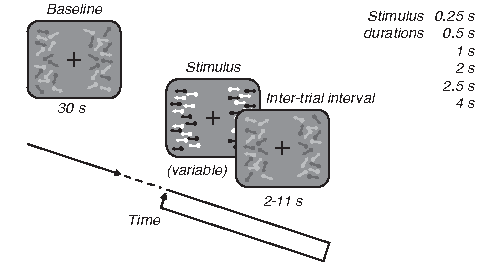
\includegraphics[keepaspectratio,width=0.5\textwidth]{figs_c1/Fig1_task.pdf}
\caption[Cortical measurement experiment.]{Cortical measurement experiment. Observers were shown patches of moving dots that increased in contrast and motion coherence on each trial. A 30-s baseline period preceded each scan with 25\% contrast dots and incoherent motion and the baseline dots persisted between trials. On each trial the contrast increased by 0, 25, 50, or 75\% and the coherence by 0, 25, 50, 75, or 100\% for a stimulus duration of 250 to 4,000 ms. Observers performed an asynchronous task at fixation throughout the experiment.}
\label{fig:c1f1}
\end{figure}

Measuring cortical responses to contrast and motion coherence.
We characterized human cortical responses to changes in contrast and motion coherence of patches of dynamic random-dot stimuli by measuring BOLD responses while observers passively viewed two patches of moving dots (Fig. \ref{fig:c1f1}). Each scan began with 30 s of baseline stimulus presentation (0\% coherence, 25\% contrast) after which trials consisting of brief increments (0.25–4 s) in either or both coherence and contrast before returning back to baseline for a random length intertrial interval (2–11 s) (see methods for full details). In total observers were shown 40 conditions: 20 consisted of combinations of changes in contrast (+0, +25, +50, and +75\%) and changes in motion coherence (+0, +25, +50, +75, and +100\%) for 2,500 ms each, the remaining 20 were a subset of these combinations combined with variable stimulus durations (250, 500, 1,000, 2,000, and 4,000 ms). To minimize task-dependent effects and maintain a consistent level of engagement, observers performed an independent fixation task during viewing. We computed hemodynamic responses to each stimulus condition for each observer using an event-related analysis for retinotopically defined visual areas V1, V2, V3, hV4, V3A, V3B, V7, and MT. We begin by describing responses in visual areas V1 (Fig. 2A) and MT (Fig. 2B), as they are well known to be sensitive to contrast \citep{Avidan2002-jg,Boynton1996-ff,Gardner2005-pg,Logothetis2001-kk,Olman2004-dd} ( Tootell et al. 1995, 1998) and motion coherence \citep{Britten1993-oh,Handel2007-xk,Rees2000-ul} (Simoncelli and Heeger 1998), respectively.


\begin{figure}
\centering
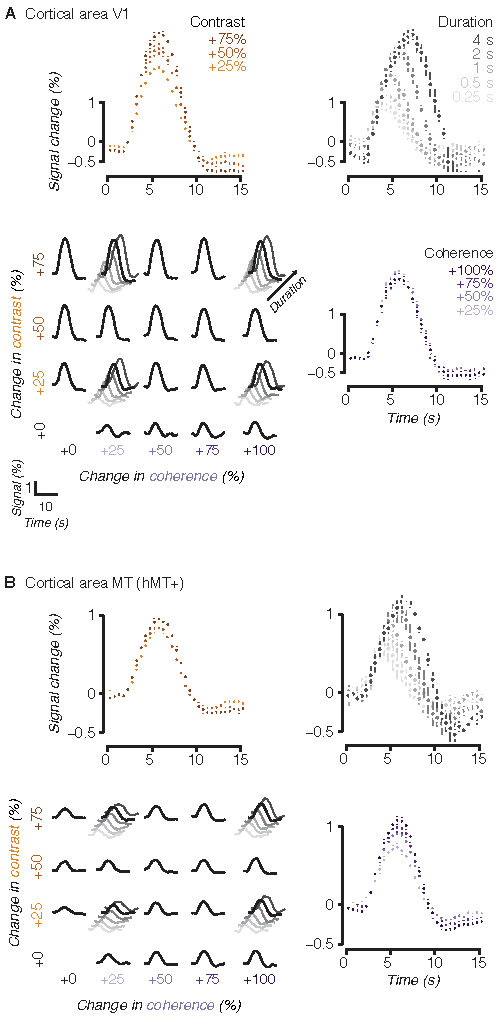
\includegraphics[keepaspectratio,width=0.5\textwidth]{figs_c1/Fig2_v1mt.pdf}
\caption[Measurements of event-related responses in cortical areas V1 and MT]{Measurements of event-related responses in cortical areas V1 and MT. A: cortical area V1. To obtain the individual responses shown here we performed an event-related analysis on our time series. In total we included 40 conditions in the experiment: 20 consisted of a full cross of changes in contrast and/or coherence presented for 2,500 ms (shown in bold in the grid in the bottom left) and 20 were a subset of the full cross conditions presented for various durations (shown in diagonal for the four conditions with additional durations recorded). We measured cortical responses to changes in contrast (top left) where each trace is averaged over changes in coherence, i.e., each response is the average of a row in the bottom left grid. We also measured responses to changes in coherence (bottom right), each trace is averaged over changes in contrast, i.e., each response is the average of a column in the grid. We made additional measurements across a large range of stimulus durations (top right) also shown in the grid. B: as in A for cortical area MT (hMT+). In all panels the event-related responses are averaged across observers and error bars indicate the bootstrapped 95\% confidence interval; some error bars may be hidden. Note that for visualization event-related responses are only shown out to 15 s but the analysis used a window of 40.5 s.}
\label{fig:c1f2}
\end{figure}

We observed clear parametric sensitivity to increases in contrast in V1 but weaker sensitivity in cortical area MT. Our measurements in V1 confirm previous results \citep{Gardner2005-pg,Logothetis2001-kk} (Tootell et al. 1995, 1998). The contrast sensitivity of V1 can be appreciated as monotonically increasing response magnitudes for higher levels of contrast increments (top left orange traces, Fig. \ref{fig:c1f2}A). These traces are for a stimulus duration of 2.5 s collapsing across motion coherence increments, i.e., averaging each row in the full response grid. While MT was also sensitive to increments of contrast, the monotonic increase appeared less pronounced compared with V1 (top left orange traces, Fig. \ref{fig:c1f2}B), consistent with other reports that have noted MT as having near maximal responses to small changes to contrast (Sclar et al. 1990; Tootell et al. 1995).

For motion coherence, we found the opposite pattern: MT was much more sensitive to increments in motion coherence compared with V1. MT showed clear monotonic increasing responses with increasing motion coherence (bottom right purple traces, Fig. \ref{fig:c1f2}B). These traces are again for a stimulus duration of 2.5 s averaged over contrast increments, i.e., collapsing each column in the full response grids. In V1 there was little difference in response amplitude as a function of motion coherence, i.e., weak sensitivity to coherence (bottom right purple traces Fig. \ref{fig:c1f2}A).

While V1 showed little parametric sensitivity to difference in coherence and MT little sensitivity to difference in contrast, both show a large response to the smallest increment of these parameters. This consistent trial-by-trial response, which we call the stimulus-onset response, appears unrelated to our parametric manipulations. For example, despite showing little sensitivity to different levels of coherence all of the responses for V1, including the one induced by the least change in coherence (+25\%), induced a large response relative to the baseline (purple traces, Fig. 2A). Similarly, for MT and contrast as can be appreciated by noting that increasing contrast by 25\% (orange traces, Fig. 2B) resulted in a large response. Part of this apparently large response is due to the fact that these responses for contrast or coherence are averaged over changes in the other parameter. That is, increases in contrast are shown averaged over coherence and vice versa. However this is not the complete story as can be appreciated by examining the grid of responses to each parameter separately (small bold black traces in grid, Fig. 2A and B). V1 can be seen to respond to a small change in coherence (+25, along horizontal) when there is no change (+0, along vertical) in contrast and vice versa for MT. These relatively large responses, to a feature each area is not strongly sensitive to, suggests that there is a response to stimulus onset regardless of condition.

Motion visibility is also adjusted by reducing the duration of stimuli, often in conjunction with reduced contrast and coherence. Along with the measurements described above, for which the stimulus duration was 2.5 s, we tested a large array of different durations from 0.25 to 4 s. As expected of an approximately linear system \citep{Boynton2012-xy} we observed that responses scaled with stimulus duration in both cortical areas V1 and MT (top right gray traces, Fig. \ref{fig:c1f2}A,B).

\begin{figure}
\centering
\includegraphics[keepaspectratio,width=\textwidth]{figs_c1/Fig3_v2v7.pdf}
\caption[Measurements of event-related responses in cortical areas V2\textemdash V7]{Measurements of event-related responses in cortical areas V2\textemdash V7. A\textemdash F: conventions are the same as in Fig. \ref{fig:c1f2}}
\label{fig:c1f3}
\end{figure}

Across the rest of the visual areas that we were able to retinotopically define in all subjects (V2, V3, hV4, V3A, V3B, and V7) we found similar parametric sensitivity to contrast, motion coherence and stimulus duration (Fig. \ref{fig:c1f3}). In general, and in concordance with previous reports \citep{Avidan2002-jg} we found less parametric sensitivity to changes in contrast for visual areas higher up in the visual hierarchy in the range we measured (+25 to +75\% contrast). Sensitivity to coherence was observed in a number of the visual areas, although MT and to a lesser extent V3A were the clear stand-outs in showing monotonically increasing responses to this parameter. These observations will be quantified below.

\begin{figure}
\centering
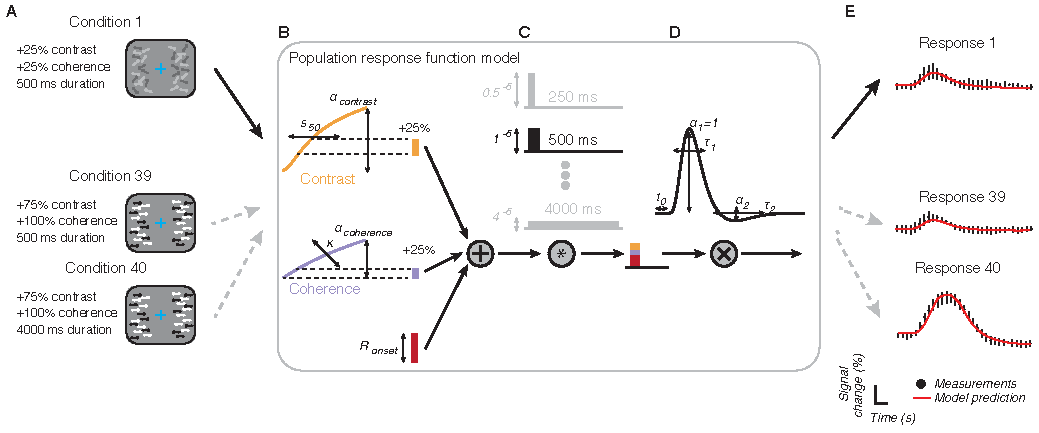
\includegraphics[keepaspectratio,width=0.5\textwidth]{figs_c1/Fig4_model.pdf}
\caption[Population response function model]{Population response function model. A: Each condition in the experiment was defined by three parameters: the increment in contrast above baseline (+0, +25, +50, or +75\%), the increment in coherence above baseline (+0, +25, +50, +75, +100\%), and the stimulus duration (250, 500, 1,000, 2,000, or 4,000 ms). As an example we use condition 1 to demonstrate the model. B: to estimate the response to each feature within a condition we first find the change in response due to the corresponding change in stimulus intensity according to the population response functions. For contrast the population response function is a Naka-Rushton with two free parameters: αcontrast controlling the amplitude and σ the shape. For coherence the response function was a saturating non-linearity with two free parameters: αcoherence controlling the amplitude and κ the shape. We added the resulting change in response together (while testing for interaction effects, see methods) and included an onset parameter to account for stimulus response that did not vary parametrically with the stimulus features. C: the total response, including onset, was used to scale a boxcar function whose length matched the stimulus duration. The boxcar was additionally scaled by a parameter to account for the nonlinear effect of stimulus duration. D: the resulting boxcar was convolved with a canonical hemodynamic response function fit separately for each observer. E: the model outputs a prediction for each condition about the expected event-related response (red lines). The parameters within the population response function model were then optimized to minimize the sum of squared errors between the data (black markers) and the model responses.}
\label{fig:c1f4}
\end{figure}

Fitting population response functions to cortical responses.
To quantify the parametric sensitivity to contrast and coherence of each visual area we fit the event-related responses with a population response model using idealized functional forms for the relationship between contrast and coherence and neural response (Fig. \ref{fig:c1f4}). Based on previous work we expected that the population response to contrast would be a sigmoidal function (Albrecht and Hamilton 1982; Sclar et al. 1990; Boynton et al. 1999) with the form of a Naka-Rushton equation (Fig. 4B, orange curve) (Naka and Rushton 1966). To avoid overfitting, we fixed the exponents in the equation based on previous work (Boynton et al. 1999) and only allowed σ and αcontrast to vary. For motion coherence, we allowed for a functional form that can smoothly interpolate between linear (Britten et al. 1992, 1993; Simoncelli and Heeger 1998; Rees et al. 2000) and a saturating exponential (Fig. \ref{fig:c1f4}B, purple curve). Finally, we included an onset term to capture the portion of response that did not vary across all conditions which presumably reflects stimulus onset and not parametric variation of stimulus parameters.

To predict the BOLD response from the modeled contrast and coherence response functions, we employed a linear-systems approach (Heeger et al. 2000; Rees et al. 2000; Logothetis et al. 2001). To account for different durations of stimuli, we multiplied the response magnitude predicted by the onset, contrast, and coherence functions with a boxcar function of appropriate length (Fig. \ref{fig:c1f4}C). As it is known that brief stimuli evoke response larger than expected by linearity (Boynton et al. 1996, 2012), we also scaled the boxcar magnitude with an exponential that accounted for this nonlinearity in response. This scaled boxcar was then convolved with a hemodynamic response function (Fig. \ref{fig:c1f4}D) whose parameters were adjusted to best fit the event-related responses across all conditions (Fig. \ref{fig:c1f4}E). All together, we fit the model parameters for the contrast function ($\alpha_{con}$, $\sigma$), coherence function ($\alpha_{coh}$, $\kappa$) and temporal effects (δ, Ronset), and the parameters for the hemodynamic response function ($t_0$, $\tau_0$, $t_1$, $\tau_1$, $\alpha_1$) for each observer for each visual area by minimizing the sum of least squares between the output of the model and the event-related responses for each of the 40 conditions.

We report the main fit parameters of the hemodynamic response function and population response function model across cortical areas (Table \ref{tbl:c1t1}) and observers (Table \ref{tbl:c1t2}). We assessed whether between-observer variability existed by fitting a linear model predicting each parameter with observers as categorical predictors and used the same procedure to assess for within-observer variability across cortical areas (see methods). We found that there was statistically significant between-observer variability across all of the parameters but only significant variability within-observer (i.e., across cortical areas) for the shape parameter of the hemodynamic response τ, the magnitude and shape parameters of the contrast response function αcontrast and σ, the parameters of the coherence response function αcoherence and κ, and the onset parameter Ronset (significance established by a partial F-test comparing linear regression models with and without each group of additional parameters at the P = 0.05 threshold). Note that the κ and αcoherence parameters which together control both the shape and magnitude of the coherence response are hard to interpret in isolation.

\begin{table}[]
\scriptsize
\begin{tabular}{|c|c|c|c|c|c|c|c|c|}
\hline
     & \multicolumn{3}{c|}{Hemodynamic response}                                                     & \multicolumn{2}{c|}{Contrast}                                                                                                     & \multicolumn{2}{c|}{Coherence}                  & Onset                                                                     \\ \hline
Area & $tau_0$     & $tau_1$*                                                         & $\alpha_1$   & $\alpha_{con}$*                                                 & $\sigma$*                                                       & \$\textbackslash{}alpha\_\{coh\} & $\kappa$     & $R_{onset}$*                                                              \\ \hline
V1   & 0.51 (0.05) & 1.80 (0.42)                                                      & -0.24 (0.06) & 1.68 (1.18)                                                     & \begin{tabular}[c]{@{}c@{}}0.35 (0.14)\\ (p=0.006)\end{tabular} & 13.94 (32.04)                    & 2.11 (6.79)  & \begin{tabular}[c]{@{}c@{}}0.42 (0.24)\\ (p\textless{}0.001)\end{tabular} \\ \hline
V2   & 0.52 (0.06) & 1.79 (0.44)                                                      & -0.24 (0.08) & 0.69 (0.57)                                                     & 0.40 (0.13)                                                     & 21.27 (27.42)                    & 0.40 (1.06)  & 0.28 (0.16)                                                               \\ \hline
V3   & 0.52 (0.07) & 1.79 (0.59)                                                      & -0.24 (0.09) & 0.63 (0.34)                                                     & 0.43 (0.13)                                                     & 13.23 (26.11)                    & -0.61 (3.13) & \begin{tabular}[c]{@{}c@{}}0.30 (0.12)\\ (p=0.013)\end{tabular}           \\ \hline
V4   & 0.52 (0.07) & 1.83 (0.93)                                                      & -0.24 (0.09) & 0.61 (0.24)                                                     & 0.47 (0.12)                                                     & 14.05 (22.42)                    & -1.83 (5.98) & 0.21 (0.13)                                                               \\ \hline
V3A  & 0.52 (0.07) & 1.79 (0.59)                                                      & -0.24 (0.09) & 0.35 (0.26)                                                     & 0.48 (0.11)                                                     & 3.41 (12.46)                     & 1.05 (1.71)  & \begin{tabular}[c]{@{}c@{}}0.15 (0.1)\\ (p=0.005)\end{tabular}            \\ \hline
V3B  & 0.52 (0.07) & 1.79 (0.59)                                                      & 0.24 (0.09)  & \begin{tabular}[c]{@{}c@{}}0.24 (0.13)\\ (p=0.003)\end{tabular} & 0.43 (0.17)                                                     & 7.99 (16.15)                     & 0.29 (0.41)  & \begin{tabular}[c]{@{}c@{}}0.14 (0.06)\\ (p=0.002)\end{tabular}           \\ \hline
V7   & 0.52 (0.07) & \begin{tabular}[c]{@{}c@{}}2.15 (0.87) \\ (p=0.032)\end{tabular} & -0.23 (0.07) & \begin{tabular}[c]{@{}c@{}}0.32 (0.25)\\ (p=0.022)\end{tabular} & 0.53 (0.22)                                                     & 9.80 (14.21)                     & 1.11 (1.87)  & \begin{tabular}[c]{@{}c@{}}0.09 (0.07)\\ (p\textless{}0.001)\end{tabular} \\ \hline
MT   & 0.51 (0.04) & 1.81 (0.63)                                                      & -0.22 (0.09) & \begin{tabular}[c]{@{}c@{}}0.22 (0.25)\\ (p=0.001)\end{tabular} & 0.58 (0.32)                                                     & 6.87 (17.60)                     & 0.92 (1.07)  & 0.24 (0.09)                                                               \\ \hline
\end{tabular}
\caption{Variability in parameter estimates across cortical areas}
\label{tbl:c1t1}
\end{table}

Table 2. Variability in parameter estimates across observers

Enlarge table

The population response model was able to capture the majority of variance in each observer’s event-related responses and a significant portion of this explained variance was accounted for by the population response functions. We assessed variance explained as the squared correlation between the model predictions and the actual event-related responses for held-out conditions. For V1, r2 = 0.69, 95\% CI [0.63 0.75]; V2, r2 = 0.63, 95\% CI [0.58 0.68]; V3, r2 = 0.62, 95\% CI [0.56 0.68]; hV4, r2 = 0.44, 95\% CI [0.35 0.53]; V3A, r2 = 0.42, 95\% CI [0.35 0.50]; V3B, r2 = 0.38, 95\% CI [0.31 0.46]; V7, r2 = 0.32, 95\% CI [0.24 0.40]; MT, r2 = 0.49, 95\% CI [0.43 0.56]. Part of the variance accounted for by the model is simply due to the stimulus-onset term and hemodynamic response, but the population response functions also captured significant variance. We assessed this by comparing our results to a model fit to the same measurements but where the condition labels were permuted. This corresponds to keeping the variance explained by stimulus onset and the hemodynamic response but randomizes the relationship between condition and response. We repeated this permutation test procedure 100 times per observer and cortical area. On average across observers and areas the variance explained by fitting to the measured data set (average cross-validated r2 = 0.508) exceeded the variance explained in the permuted data set (average cross-validated r2 = 0.340) with P < 0.001, Δr2 = 0.164, 95\% CI [0.162 0.165].

Across cortical visual areas the model captured the response to changes in contrast and motion coherence as well as the amplitude effects due to duration. To visualize the fit of the population model to each variable we scaled the canonical hemodynamic response function for each observer to fit the event-related responses in the conditions with either no change in contrast or no change in coherence. This results in a single scaling factor for each of these conditions (circles, Fig. 5) which we compared with the model predictions (lines, Fig. \ref{fig:c1f5}). Examination of the magnitude of the population model fit to the event-related response peaks for changes in contrast (orange curves, Fig. 5A) and coherence (blue curves) shows good correspondence. This is particularly notable given that the model is fit across all conditions containing different response lengths, as well as combinations of contrast and coherence changes, while the displayed data are for changes in contrast and coherence in isolation. This visualization displays a model fit to all the data, i.e., not on held-out data, but with similar explained variance to the cross-validated model (difference between cross-validated and full fit, $\Delta r^2=$=0.005, 95\% CI [0.004 0.006]). The population response functions echoed the qualitative results described above for the event-related responses: V1, V2, V3, and hV4 showed strong response to contrast with relatively weak response to coherence. Only MT showed stronger response to motion coherence than to contrast. Moreover, the amplitude of responses as a function of duration (Fig. \ref{fig:c1f5}B) were similarly well captured by the population response model. As noted earlier the amplitude of responses due to doubling in duration do not appear to scale in a linear manner.


\begin{figure}
\centering
\includegraphics[keepaspectratio,width=0.5\textwidth]{figs_c1/Fig5_fit.pdf}
\caption[Population response functions.]{Population response functions. A: the population response functions fit to each cortical area V1-MT (hMT+) are shown compared with the magnitude of the event-related response for the conditions in which only one feature changed. These correspond to the conditions in the first column and last row of each event-related response grid in Figs. 2 and 3. To make the functions comparable to the data in an easy to interpret space we reduced each event-related response to a single magnitude value which was obtained by finding the linear scaling of the canonical hemodynamic response to that condition. The model outputs predictions for all 40 conditions but we are only showing the subset where either contrast or coherence changed alone. Note that the predictions here are not out of sample (i.e., these are not the cross-validation results) but we show the full fit to better visualize the response functions. B: as in A but for the variable duration conditions in which contrast and coherence changed maximally (+75\% contrast, +100\% coherence). In all plots markers indicate the average across observers and error bars the bootstrapped 95\% confidence interval.}
\label{fig:c1f5}
\end{figure}


The form of the contrast response function has been extensively studied \citep{Albrecht1982-rq,Boynton1999-jd,Sclar1990-lk} while the motion coherence response function has received much less attention. Single-unit studies have found a linear response function, whereas BOLD measurements in humans have found some non-linearity of response, particularly outside of MT \citep{Rees2000-ul}. We therefore tested for non-linearity in the population response functions to motion coherence and found that responses were generally best characterized as linear, with a small deviation from linearity for MT. We quantified this comparison as the difference in cross-validated variance explained between the saturating exponential and a linear form for the coherence response function. In MT we found a small difference in favor of the nonlinear model Δr2 = 0.004 (95\% CI [0.001 0.007]) while all other cortical areas’ confidence intervals overlapped with zero. This difference is visible as the saturation of the MT coherence response to large changes in coherence (Fig. 2B and Fig. 5A, MT).

While population responses to each motion feature could interact, i.e., a change in contrast might influence the response to a change in coherence or vice versa, we found no evidence for this. We tested for interactions by adding an additional beta weight to the model accounting for the effect of multiplicative changes in contrast and coherence (see methods section Population responses: functional forms). Including this term reduced the cross-validated variance explained by on average −6.67\% (95\% CI [−13.42, 0.08]) across cortical areas, suggesting overfitting compared with the no-interaction model. One observer’s data was particularly strongly overfit. Removing that observer resulted in an average reduction in variance explained of −0.08\% (95\% CI [−0.25 0.09]) and for individual areas, V1: −0.18\%, V2: −0.16, V3: −0.17, hV4: −0.13, V3A: −0.07, V3B: −0.14, V7: −0.07, MT: −0.11.

Visual inspection of the response grids (bottom left panels in Fig. 2 and 3) suggest an alternative kind of interaction in which the response to contrast and coherence might be stronger in the absence of the other feature changing. Take for example the response to contrast compared with coherence in V1. The contrast response in V1 is so much larger than the response to coherence that it’s possible it “washes out” any visible effect due to coherence. To test for this possibility we fit a model with different population response functions for conditions in which only a single feature changed vs. when both features changed. We found that these models were also not statistically better than the simplest model with no interactions: average reduction in cross-validated variance explained −5.34\% 95\% CI [−9.13, −1.56] and without the overfit observer −0.20\% 95\% CI [−0.31, −0.08]. Although statistically the models were similar in our data set we did find that in the interaction model the population response functions to contrast had a higher maximal response when the coherence was not simultaneously changed, but the reverse was not true. On average across subjects and cortical areas we found an increase in sensitivity of ~50\% in the contrast response when no simultaneous change in coherence occurred (average parameter change 1.68 95\% CI [0.58, 2.78], significantly different from zero as assessed by bootstrap over observers, P = 0.007).

The population response model fits (Fig. 5) replicate earlier reports showing that contrast responses have a smaller dynamic range and saturate more quickly in higher visual cortical areas (Avidan et al. 2002), and add the finding that coherence sensitivity peaks in MT. To assess this we plotted the maximum of the contrast response function (the αcontrast parameter) against the linear slope of the coherence response function (the response range measured as the slope of a linear fit, see methods) for each cortical area (Fig. 6A). As expected we found stronger sensitivity to motion coherence in V3A and MT compared with area V1 (Dupont et al. 1994; Tootell et al. 1995; Watson et al. 1993; Zeki et al. 1991). The difference in coherence sensitivity between V3A and V1 was 0.167, P < 0.001 and between MT and V1 0.251, P < 0.001. But we also observed significant sensitivity to changes in coherence in all regions measured (Fig. 6B): V1 = 0.12, V2 = 0.19, V3 = 0.18, hV4 = 0.13, V3A = 0.25, V3B = 0.15, V7 = 0.22, MT = 0.36, slopes in \% signal change/unit coherence, all P < 0.001 assessed by bootstrap across observers. All cortical visual areas showed statistically significant parametric sensitivity to changes in contrast (Fig. 6C) assessed as a nonzero αcontrast parameter by bootstrap across observers, all P < 0.001 except MT, P = 0.002. The maximum contrast response dropped quickly for regions higher in the visual hierarchy (V1 = 2.00, V2 = 0.87, V3 = 0.68, hV4 = 0.63, V3A = 0.35, V3B = 0.24, V7 = 0.33, MT = 0.20, units in \% signal change/unit contrast).


\begin{figure}
\centering
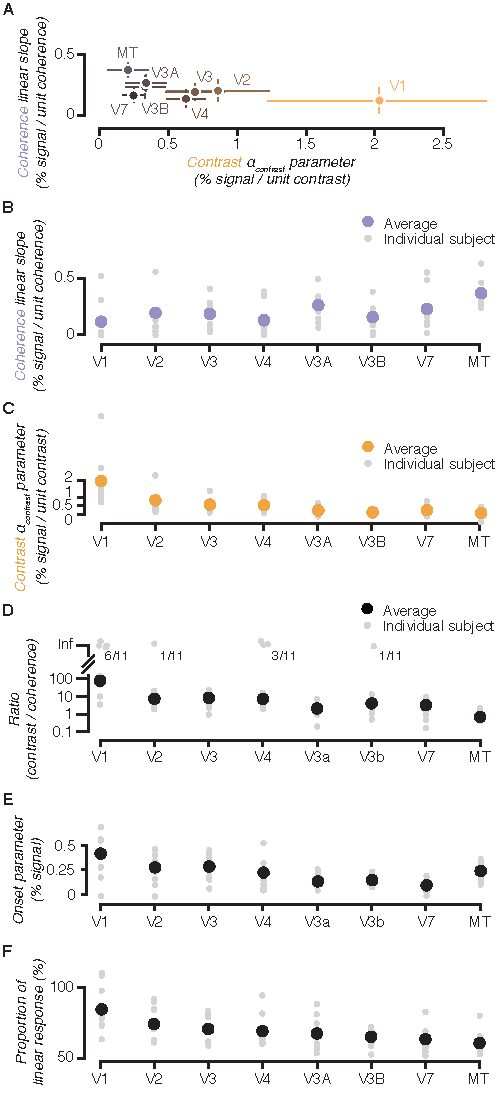
\includegraphics[keepaspectratio,width=0.5\textwidth]{figs_c1/Fig6_sensitivity.pdf}
\caption[Cortical sensitivity to contrast and motion coherence]{Cortical sensitivity to contrast and motion coherence. A: to obtain a qualitative estimate of cortical sensitivity to each motion visibility feature across the cortical visual areas we plotted the αcontrast parameter from the Naka-Rushton function against the slope of a linear fit of the coherence functions. B: the slope of the coherence functions fits as in A replotted with individual subjects. C: the αcontrast parameter as in A replotted with individual subjects shown for each cortical area. D: we plot the ratio of the sensitivity parameters as an unbiased additional comparison because the amplitude parameters could be sensitive to the signal-to-noise ratio of the measurement in different cortical areas. Note that for some subjects the slope of the coherence response was near zero in some cortical areas, we note these as a ratio of infinity (Inf). The means are calculated excluding infinite values. E: the stimulus-onset response parameter $R_{onset}$ indexes the portion of the response that was not parametrically modulated by contrast or coherence. F: for each doubling in stimulus duration the proportion of response increase is shown by cortical area where 100\% would indicate that responses increased linearly with duration. In all panels markers indicate the mean and error bars the bootstrapped 95\% confidence interval. Error bars are omitted in panels (B–E) for visualization.}
\label{fig:c1f6}
\end{figure}

Although we fit a Naka-Rushton function to the contrast response our measurements were limited to only a few points (no change in contrast, +25, +50, and +75\%). This meant that the data did not strongly constrain a sigmoidal fit. We assessed whether in our data set the results would be equally well fit by a linear model and found that this was the case for all areas except V7, with an average improvement of 0.32\% in cross-validated variance explained. Therefore, the αcontrast parameter which fits the maximal response to contrast in each region tracks the slope of the relationship between contrast and response and can therefore be used as a measure of the sensitivity to contrast, in the range of contrasts we measured. The linear model’s improvement in variance explained for individual areas were V1 0.66, 95\% CI [0.16 1.15]; V2 0.79, 95\% CI [0.14 1.45]; V3 0.51, 95\% CI [0.04 0.98]; V4 0.27, 95\% CI [0.09 0.45]; V3a 0.24, 95\% CI [0.06 0.42]; V3b 0.17, 95\% CI [0.03 0.31]; V7 −0.04, 95\% CI [−0.14 0.06]; MT 0.21, 95\% CI [0.07 0.34].

We found that the variability in our measurements did not differ significantly across different cortical areas or according to the stimulus strength. We performed this analysis to test whether various nuisance variables could have altered our measurements, e.g., proximity to the coils and partial voluming might affect signal-to-noise in different cortical areas, or the variability in our measurements might increase with response magnitude as contrast and coherence cause populations of neurons to be more active. To do this we estimated the response magnitude of every trial and grouped these by condition and cortical area, then fit a series of linear models to see whether variability differed. We found that none of the additional variables improved the model fit over the intercept-only model at the P = 0.05 significance threshold. Importantly, the model that allowed separate values for each cortical area did not improve the model fit, suggesting that response variability did not significantly differ between cortical areas (mean cortical area standard deviation was 1.50 percent signal change; V1 1.75, 95\% CI [1.33 2.17]; V2 1.08, 95\% CI [0.91 1.25]; V3 1.28, 95\% CI [1.06 1.49]; V4 1.37, 95\% CI [1.03 1.72]; V3a 5.71, 95\% CI [1.28 10.15]; V3b 1.14, 95\% CI [0.96 1.31]; V7 1.32, 95\% CI [0.97 1.66]; MT 1.30, 95\% CI [0.95 1.66]). In addition we found that there was no statistically significant change in variability in the slope of the relationship between variability and stimulus strength (even when separate slopes were allowed for different cortical areas), suggesting that noise in our measurements was additive, i.e., did not increase with increasing response magnitude. Fitting the model with a slope for contrast and coherence (shared across areas) results in a slope of −1.23 percent signal change per unit contrast, t(2,557) = −1.27, P = 0.21, and a slope of −0.58 percent signal change per unit coherence, t(2,557) = −0.78, P = 0.44.

Although our measurements do not suggest that any bias is introduced by potential signal-to-noise differences across areas, we computed the ratio of the contrast and coherence slope parameters as an additional unbiased analysis (Fig. 6D). This ratio allows for between region comparison of the sensitivity to contrast and coherence because the ratio reports how sensitive each region is to contrast compared with coherence and not overall sensitivity. That is, the ratio should be invariant to differences in signal-to-noise, under the assumption that contrast and coherence sensitivity are equally affected. In line with our previous results we found that V1 has a ratio of contrast to coherence sensitivity that is at least an order of magnitude more than the other areas. In addition MT was found to have a ratio near 1 and lower than the other cortical areas, reflecting its stronger relative sensitivity to coherence.

We found that the portion of the BOLD response that did not vary parametrically with contrast or coherence, the stimulus-onset response Ronset did vary across cortical areas (Fig. 6E and Table 1). On average the onset response was 0.23 percent signal change across observers and cortical areas. The stimulus-onset response in V1 and V3 were larger than average at 0.42 percent signal change, 95\% CI [0.28, 0.55], while areas V3A, V3B, and V7 were smaller than average, 0.14, 95\% CI [0.07, 0.20]; 0.15, 95\% CI 0.11, 0.18]; 0.09, 95\% CI [0.06, 0.13], respectively. The other cortical areas’ onset effects were V2 0.28, 95\% CI [0.19, 0.37]; V3 0.22, 95\% CI [0.22 0.36]; V4 0.23, 95\% CI [0.15, 0.31]; MT 0.24, 95\% CI [0.19, 0.29].

Finally, we found that the effect of increasing stimulus duration was not consistent across cortical areas (Fig. 6F). We found that early visual cortex, V1 in particular, was significantly more sensitive to changes in duration than later visual areas, especially MT. The effect of a doubling in duration on the population response, as a proportion of that expected from a linear model, was 68.56\%. On average across subjects we found that V1 and MT differed significantly from the average. We found that the effect of a doubling in duration in V1 was 83\% of the linear model, 95\% CI [76.00, 92.27], suggesting that V1 is more sensitive to stimulus duration. By contrast in MT the effect was only 62\% of the linear model, 95\% CI [57.06, 66.08], suggesting that MT may have a more transient response. The effects in other areas were not significantly different from the average: V2 73\%, 95\% CI [67.20, 79.70]; V3 70\%, 95\% CI [65.05, 74.95]; V4 70\%, 95\% CI [64.21, 76.59]; V3A 67\%, 95\% CI [61.24, 73.31]; V3B 64\%, 95\% CI [60.45, 67.64]; V7 64\%, 95\% CI [58.07, 70.02].

\section{Discussion}

We have developed a quantitative framework for modeling human cortical response to motion visibility as parameterized by image contrast, motion coherence, and duration. Our results provide a comprehensive view of the variability in cortical sensitivity to these features, each of which is a critical component of visual stimuli often manipulated in experiments designed to understand visual perception and decision-making. Our measurements show that the range of responses to different levels of contrast was larger in early visual cortex, especially V1, and the range of responses for coherence larger in V3A and MT (hMT+). Nonetheless, a change in either feature caused a cortical response in all the retinotopic areas we mapped. Our results weigh on various other findings in the literature: the precise shape of population response functions, the influence of stimulus duration on cortical signals, and whether or not sensory representations for different features interact. Finally, we believe that this parameterized model, and parametric models in general, suggest mechanisms for the read out of sensory representations from population responses and have therefore made our measurements and framework available online as a resource (see methods).

We studied changes in contrast, coherence, and duration to measure human cortical response within a range where typical human perceptual experiments are performed. One choice we made was to measure contrast from a relatively high baseline. Because the contrast response function is known to adapt to the current background stimulus without altering the form of parametric modulation (Ohzawa et al. 1982, 1985; Sclar et al. 1985, 1989; Gardner et al. 2005) the relative sensitivities we measured should hold at other baselines. With this design we were also able to show that sensitivity to changes in contrast and coherence do not interact. The interaction analysis would be impossible in stimuli where the dots appear from a black or gray background such that both contrast and coherence always change together (Britten et al. 1993; Rees et al. 2000). When designing the dot motion stimulus we also had to ensure that there were sufficient dots and a large enough aperture to be clearly visible and generate a reliable coherence response. At low dot densities the response to changes in coherence are negligible (Smith et al. 2006) and small aperture sizes can cause changes in coherence to result in decrements in response (Ajina et al. 2015; Becker et al. 2008; Costagli et al. 2014). By creating a large stimulus with high density we guaranteed that our dot motion would blanket the population receptive fields of all the cortical areas measured.

We set our stimulus to move at a constant rate of 6°/s, within the peak range of speed tuning in visual cortex, and used a dot stimulus rather than gratings to avoid having spatial frequency tuning affect our measurements. Although individual V1 and MT neurons in the macaque differ greatly in their speed tuning the average tuning of the population is quite similar and centered near 6°/s with ranges that extend far above and below that \citep{Priebe2006-uy}. Measurements of speed tuning in humans evidence broad variability across all of visual cortex but our chosen speed is within the peak range \citep{Singh2000-wr,Hammett2013-fg}. One common concern with speed tuning in gratings is that spatial frequency tuning differs across cortex and directly impacts sensitivity to other stimulus properties, such as image contrast \citep{Priebe2003-ua,Priebe2006-uy}. We used a random dot stimulus with a wide range of spatial frequency components rather than gratings with a specific spatial frequency to avoid this confound. In principle our stimulus drives neurons with a wide range of tunings and by averaging over voxels in each cortical area we reduce the impact of columnar and other local microstructure in each area \citep{Sun2007-cf}(Liu and Newsome 2003).

We reported here several parameters which together defined the population response functions, but which of these represents a good measure of the sensitivity of a region? We use the term sensitivity to capture parametric differences in response magnitude with differences in contrast or coherence. Thus, an area with high contrast or coherence sensitivity is one in which the response to the lowest and highest values of these parameters evoke the largest difference in response (see methods for how the reported parameters correspond to this). This measure can be used to compare with human behavioral contrast or coherence discrimination performance since signal detection theory predicts that perceptual sensitivity, d′, is directly proportional to this difference (Boynton et al. 1999; Newsome et al. 1989; Pestilli et al. 2011; Tolhurst et al. 1983; Zenger-Landolt and Heeger 2003). However, d′ is also inversely proportional to the standard deviation of response which could vary across different areas, particularly for measurement related reasons that would therefore distort our measures of sensitivity. Our analysis of the variability of response across different areas did not find differences, thus suggesting that our measures are an accurate reflection of contrast and coherence sensitivity. Moreover, we used a selection criterion to analyze a subset of voxels that show consistent trial-to-trial responses to reduce the effect of measurement noise but our parametrization will still be sensitive to any noise that remains.

Response variability might also change with response amplitude as it is known to do for single-unit responses. Although occasionally single neurons can be found that match perception (Britten et al. 1992), groups of neurons (Tolhurst et al. 1983) or larger populations (Averbeck et al. 2006; Zohary et al. 1994), depending on the correlation structure in the population, are likely to more closely reflect perceptual reports. Supporting the idea that populations are used for perceptual readout is evidence from human work where at the coarse resolution of the BOLD signal, which pools over large numbers of neurons, cortical measurements closely track perception under an assumption of additive noise (Boynton et al. 1999; Hara and Gardner 2014; Pestilli et al. 2011; Sapir et al. 2005). In line with this the variance of population responses measured with voltage-sensitive dyes do not change with magnitude of response in V1, i.e., they are additive (Chen et al. 2006). Our own measurements support the hypothesis that populations are subject to additive noise: we found that as contrast and coherence increased and caused larger magnitudes of response we found no evidence that trial-by-trial variability changed. Together our data and previous results suggest that measures of the slope in the BOLD signal population response function are indeed measures of sensitivity and leaves us with a testable prediction: if parameters measure sensitivity (i.e., signal-to-noise ratio) then they should be relatable to human perception under additive noise but not noise which scales with response magnitude.

We observed a saturation of the cortical response to motion coherence that differs from recordings of a linear response in MT in human (Händel et al. 2007; Rees et al. 2000) and monkey (Britten et al. 1993). Saturation of the contrast response function is thought to be the result of normalization, a canonical computation in cortex (Baker and Wade 2017; Carandini and Heeger 2012). If the response to motion coherence is linear, it might suggest that similar normalization does not apply. In fact, models of the V1 to MT circuitry include explicit normalization (Simoncelli and Heeger 1998) and the normalization strength alters whether the model predicts linear or saturating responses. This may account for the discrepancies of results; i.e., normalization may result in weak saturation of coherence response as we have found, in line with evidence from both humans (Costagli et al. 2014; Rees et al. 2000) and monkeys (Britten et al. 1993). In support of this idea is evidence that in the absence of a normal input from V1 the coherence response function in MT becomes more linear, possibly reflecting an increased input from subcortical regions whose coherence response is linear (Ajina et al. 2015). To clarify this we can again turn to behavior. Because the MT response has been linked to behavior (Katz et al. 2016) our model makes a testable prediction: under the assumption that the visual system performs signal detection subject to additive noise (Boynton et al. 1999) a saturating coherence function would predict worse discriminability of coherence at higher base levels of coherence.

To build out our quantitative framework we measured responses to stimuli of varying durations, down to those typically used in psychophysical experiments (e.g., 0.25 s) as well as at durations more typically used for BOLD measurement (e.g., 4 s). Our results confirm many previous results showing that there exists a nonlinearity in the BOLD response, such that shorter stimuli have a larger response than expected by temporal linearity \citep{Boynton1996-ff,Boynton2012-xy}. Modeling our responses, we found that on average across cortical areas a doubling of the stimulus duration was associated with an increase in response of only 67\% of the expectation of a linear model. Whether or not this is due to neural adaptation \citep{Buxton2004-rg} or saturation of the BOLD signal \citep{Friston1998-bo} cannot be determined from our data. We also observed a slight difference in the duration effect across cortical areas. In V1 increasing duration results in a larger effect on the population response whereas MT showed a smaller than average response, which could be a result of the more transient response in MT \citep{Stigliani2017-oe}.

We also noted that any change in the stimulus, regardless of the type, amplitude, or duration resulted in what we refer to as a stimulus-onset response in all cortical areas. What is the nature of this response? Early recordings comparing BOLD responses to electrophysiological recording suggest that the BOLD signal may be thresholded at some minimum response even though neural activity continues to be modulated below that threshold \citep{Logothetis2001-kk}. Another possibility is that the stimulus-onset response may be the result of a consistent trial structure causing anticipatory responses \citep{Cardoso2012-cu}. In the latter case fitting a separate stimulus onset parameter to absorb this trial-structure related variance is appropriate to correctly estimate the population response from the BOLD signal.

Our approach to making a parametric model of cortical response to motion visibility contrasts with more complex models, such as Gabor wavelet pyramids and deep convolutional networks \citep{Kay2008-mj,Kay2017-bj,Yamins2014-rm} that are typically image-computable and thus can make detailed predictions of cortical response properties directly from images. A complete image-computable model would implicitly contain our parametric model within it and seemingly obviate the need to parameterize stimulus visibility and its relationship to cortical response. Building such complex models is a worthy goal, however, we would note that much success in understanding visual cortex function has come from experiments which parametrically altered visual features, in particular features related to visibility. Consider the result of stimulus combination. When two gratings with different luminance contrast are presented the evoked response is not well captured by simple rules such as linear summation or winner-take-all \citep{Busse2009-pt}. Instead, across a large range of parameter combinations the evoked response is well explained by normalization (Carandini and Heeger 2012). The canonical rule that an evoked response should be scaled by the response of a neighboring region of cortex is easily understood in a parametric model, but far less intuitive in a complex one. Another low-dimensional parametric model is the population receptive field \citep{Dumoulin2008-uc,Wandell2015-uv}, which has been widely used to map and interpret the properties of retinotopic visual cortex, largely because of its simplicity. In general, low-dimensional quantitative frameworks like the one we have built can parameterize cortical response to key stimulus properties and by doing so, serve to make testable predictions for perceptual function. For example, our framework suggests that small variation in sensitivity across cortical areas might be used to separately determine the visibility of motion for different parameters. That is, a read-out of the visual representations could take advantage of the differences in feature sensitivity by differentially weighting V1 and MT for contrast discrimination and vice versa for coherence discrimination.

Each parameter of motion visibility that we studied has been separately used to uncover the neural basis of different aspects of perception and perceptual decision making. The quantitative framework that we have proposed here shows that despite their similar effects on perception, contrast, coherence, and duration have distinct cortical representation at the level of populations. In studies of perception, the effects of these parameters on cortical response should not be considered to be interchangeable. With our reference framework one can now make changes in one parameter or the other and predict how this will affect human cortical response. In this way our predictive model is a key tool in furthering the goal of linking cortical response to perceptual behavior.

\chapter[Fixed vs. flexible readout]{Aim 3: Evaluating fixed and flexible readout as mechanisms of selective attention}

\section{Introduction}

Humans can flexibly attend to different aspects of the environment when their goals require it. This can be operationalized by asking human observers to report about one feature of a visual stimulus while ignoring other features. Such context-dependent judgments could be supported by a cortical implementation which increases sensitivity or selectivity for the sensory representations of reported features while suppressing others. A second and potentially complimentary implementation is to maintain stable sensory representations while flexibly changing the downstream readout of these. 

A great deal of evidence exists for the former possibility of changing representations to accommodate behavioral demands. Behavioral manipulations of spatial attention \citep{Klein2014-oe,Mitchell2009-do,Pestilli2011-gi,Womelsdorf2006-np}, feature-based attention \citep{Baldauf2014-uj,Harel2014-wd,Huk2000-uj,Jehee2011-mb,Serences2007-le,Cohen2013-uz,Treue1999-mp}, and stimulus expectations \citep{Kok2012-rh,Kok2013-km} all have been associated with changes in sensory representations. These changes may occur very early in the visual hierarchy \citep{Ling2015-fr} and take the form of changes in sensitivity \citep{Reynolds2000-mg,Serences2007-le,Snyder2018-yr,Treue1999-mp}, shifts in feature selectivity \citep{Cukur2013-gx,David2008-zx,Kastner1998-bi,Klein2014-oe,Spitzer1988-ib,Womelsdorf2006-np} (Reynolds et al., 1999; Womelsdorf et al., 2008), increases in baseline response \citep{Buracas2007-pe,Chen2012-ek,Kastner1999-qu,Ress2000-pa,Li2008-fe} Murray, 2008) useful for efficient selection \citep{Hara2014-tm,Pestilli2011-gi}, and changes in the structure of stimulus-driven and noise correlations (Cohen and Maunsell, 2011, 2009; Mitchell et al., 2009; Ruff and Cohen, 2016; Verhoef and Maunsell, 2017). 

However, flexible readout rather than change in sensory representation can be a behaviorally advantageous implementation of task demands. Although changing sensory representations can be beneficial, there cans be associated behavioral costs to suppressing ignored features in sensory representations \citep{Gazzaley2005-vd}  Mesgarani and Chang, 2012; Rees et al., 1997) when these are actually relevant to behavior. In many dramatic demonstrations (Haines, 1991; Mack and Rock, 1998; Neisser, 1979; Simons and Chabris, 1999) observers have been made blind to salient events when reporting about other aspects of a visual scene. This suggests a potential advantage to maintaining stable sensory representations and using flexible sensory readouts to enable adaptable behavior \citep{Bugatus2017-wl,Mante2013-tn,Peelen2009-us}.

Finding changes in sensory representations across different task conditions is not enough to demonstrate that these changes are large enough to explain perceptual behavior.  Instead, linking models are needed. Quantitative linking models (Barlow, 1972; Brindley, G. S., 1970; Cohen and Maunsell, 2010; Cook and Maunsell, 2002; Newsome et al., 1989; Pestilli et al., 2011; Teller, 1984) connect measurements of cortical activity to behavior by modeling the presumed process by which sensory activity gives rise to perceptual behavior. Such linking models are explicit hypotheses that can be falsified if they are unable to quantitatively link sensory representational changes to behavioral performance across different task conditions.

Here we used a linking model to study human reports of motion visibility and to understand whether sensory change or flexible readout implement this behavior. We first established that observers could independently report about either the contrast (luminance difference between dark and bright dots) or motion coherence (percentage of dots moving in a coherent direction) of random dot patches while ignoring the other feature. We then extended a well-established linking model of human contrast perception (Boynton et al., 1999; Foley and Legge, 1981; Gardner, 2015; Ling and Carrasco, 2006; Nachmias and Sansbury, 1974; Pestilli et al., 2009) to account for behavioral performance during these tasks. Because in individual cortical areas the response to motion visibility is mixed, we allowed the model to weight retinotopic areas according to their sensitivity to the two features. The critical step to understand behavioral flexibility was to measure BOLD signal while observers performed each discrimination task. If sensory representations changed enough, then a linking model with a fixed readout of sensory areas should account for behavior (i.e. that used the same weighting of cortical responses for both tasks). Implementing such a fixed readout model showed that sensory changes alone were insufficient in magnitude to explain perception. Instead, in addition to the sensory change, a change in readout between different task conditions was necessary (i.e. a flexible readout). A benefit of flexible readouts is that sensory representations can retain information about the unattended feature. In line with this, we show that observers can re-map their reports unexpectedly. 

\section{Methods}

\subsection{Observers}
In total 29 observers were subjects for the experiments. All observers except one (who was an author) were naive to the intent of the experiments. Eight observers were excluded during initial training sessions due to inability to maintain appropriate fixation (see eye-tracking below). All of the remaining 21 observers (13 female, 8 male; mean age 28 y; age range 18-55) performed the motion visibility behavioral experiment outside of the scanner. Observers performed up to six one-hour sessions on separate days for an average of 2467 trials each (range 1167-3652, standard deviation 497). Ten of the observers (7 female, 3 male; mean age 26 y; age range 19-36) repeated the motion visibility experiment inside the scanner. Observers were scanned in two 90-minute sessions, each consisting of eight 7-minute runs, and a third one-hour scan which included retinotopy and anatomical images. Procedures were approved in advance by the Stanford Institutional Review Board on human participants research and all observers gave prior written informed consent. Observers wore corrective lenses to correct their vision to normal when necessary.

\subsection{Hardware setup for stimulus and task control}

Visual stimuli were generated using MATLAB (The Mathworks, Inc.) and MGL (Gardner et al., 2018). During scanning, stimuli were displayed via an Eiki LC-WUL100L projector (resolution of 1920x1080, refresh-rate of 100 Hz) on an acrylic sheet mounted inside the scanner bore near the head coil. Visual stimuli were viewed through a mirror mounted on the head coil and responses were collected via an MRI-compatible button box. Outside the scanner, stimuli were displayed on a 22.5 inch VIEWPixx LCD display (resolution of 1900x1200, refresh-rate of 120 Hz) and responses collected via keyboard. Output luminance was measured for both the projector and the LCD display with a PR650 spectrometer (Photo Research, Inc.). The gamma table for each display was dynamically adjusted at the beginning of each trial to linearize the luminance display such that the full resolution of the 8-bit table could be used to display the maximum contrast needed. Other sources of light were minimized during behavior and scanning.

\subsection{Eye tracking}

Eye-tracking was performed using an infrared video-based eye-tracker at 500 Hz (Eyelink 1000; SR Research). Calibration was performed throughout each session to maintain a validation accuracy of less than 1 deg average offset from expected using either a ten-point or thirteen-point calibration procedure. Trials were canceled on-line when an observer’s eye position moved more than 1.5 deg away from the center of the fixation cross for more than 300 ms. During training and before data collection, observers were excluded from further participation if we were unable to calibrate the eye tracker to an error of less than 1 deg of visual angle or if their canceled trial rate did not drop to near zero. After training canceled trials consisted of fewer than 0.1\% of all trials. Due to technical limitations eye tracking was not performed inside the scanner. 

\subsection{Experimental design}

\subsubsection{Stimulus}

Motion stimuli consisted of two patches of random dot stimuli flanking a central fixation cross (1 x 1 deg). The random dot stimulus patches were rectangular regions extending from 3.5 to 12 deg horizontal and -7 to 7 deg vertical on either side of the fixation cross. Each patch was filled with 21 dots / deg2, 50\% brighter and 50\% darker than the gray background (300 cd / m2 in the scanner and 46 cd / m2 during behavior. All dots moved at 6 deg / s updated on each video frame. Motion strength was adjusted by changing motion coherence: the percentage of dots that moved in a common direction with all other dots moving in random directions. Dots were randomly reassigned on each video frame to be moving in the coherent or random directions. Both patches maintained a constant baseline in between trials of 25\% contrast and incoherent motion. To minimize involuntary eye movements, the coherent dot motion direction was randomized to be horizontally inward or outward from fixation on each trial, such that the two patches moved in opposite directions. 

\subsubsection{Contrast and coherence tasks}

Observers performed a two-alternative forced choice judgment about the visibility of the two dot patches (Fig. 1). At the start of each run observers were shown the word “contrast” or “motion” cueing them to report which side had the higher contrast or motion coherence, respectively. Each run began with a 5 s baseline period during behavioral measurements or 30 s during scanning (25\% contrast, 0\% coherence) to allow time for adaptation to occur. Trials consisted of a 0.5 s increment in either or both the contrast and motion coherence of the dot patches, a variable delay of 0.5 - 1 s, and a response period of 1s. The dot patches then returned to baseline for an inter-trial interval of 0.2 to 0.4 s randomly sampled from a uniform distribution (2 to 11 s, sampled from an exponential distribution during scanning). The base stimulus strength increments were chosen to be +7.5, +15, +30, and +60\% contrast above the baseline 25\% contrast and +15, +30, +45, and +60\% coherence above the baseline 0\% coherence. On every trial one dot patch was chosen as the target for contrast and incremented by an additional small delta, and the same was done independently for coherence. The target increment for the uncued feature was randomly chosen from [0.0, 1.8, 2.5, 3.5, 4.9, 6.9, 9.5, 13.3, 18.5\%] for contrast and [0.0, 5.0, 6.9, 9.6, 13.4, 18.6, 25.9, 36.1, 50.2\%] for coherence. The relevant target increment was chosen by a PEST staircase (Taylor and Creelman, 1967) to maintain ~82\% correct on the cued task for each base strength (4 base strengths x 2 task conditions = 8 total staircases). Observers indicated with a button press which side contained the delta increment of the cued feature. An observer would be at chance performance if they reported on the wrong feature. Staircases were initialized on the first run (after training) at 25\% and 85\% for contrast and coherence, respectively. The staircases were maintained across sessions, but the step size was reset to one third the threshold every third run to allow for long-term fluctuation. Before data collection observers trained on the task until their performance at all base stimulus strengths was measurable (i.e. their threshold converged to less than 1 minus the base strength), on average one hour of training. Behavioral runs lasted four minutes and observers took breaks as needed. Observers performed up to 6 one-hour sessions of behavioral runs spanning multiple days.

On a subset of the motion visibility experiment runs (two of every five runs) observers were occasionally asked to report about the non-cued feature (trial probability 1/7, randomized). We refer to these as catch trials. Stimulus presentation occurred as normal on catch trials but after stimulus presentation and a fixed 0.5 s delay, a letter replaced the fixation cross to indicate that the observer needed to recall and respond about the un-cued feature. The length of the delay periods in both catch and regular trials (0.5 s and 0.5 - 1 s, respectively) were chosen to ensure observers could not rely on iconic memory to complete the task (Sperling, 1960) and to avoid observers getting into a rhythm and responding before the post-cue could appear. On contrast runs the post-cue letter was an “M” indicating that observers should recall about motion coherence and on coherence runs a “C” to indicate contrast. To improve our statistical power in estimating perceptual sensitivity during catch runs we used a single base stimulus increment: +30\% contrast and +40\% coherence. These base increments were used both for catch and regular trials on these runs.

\subsection{Behavioral data analysis}

To assess whether the perceptual data could be well characterized by a signal detection framework we tested the fit of cumulative normal distributions to the measured psychometric functions. We collapsed data from all observers across the four base stimulus strengths and separated trials in which observers discriminated contrast or coherence. We binned data according to the difference in stimulus strength for each task and computed the probability of making a rightward choice in each bin (filled circles, Figure 2a, b). We fit the binned data with a cumulative normal distribution (three parameters: the mean, $\mu$, standard deviation, $\sigma$, and a lapse rate, λ which scaled the function so that it spanned the range λ/2 to 1-λ/2) and evaluated the cross-validated fit on a held-out observer using the pseudo $r^2$:

\begin{equation}
    r_{pseudo}^2=1 - \frac{\log(\mathcal{L}_{model})}{\log(\mathcal{L}_{null})}
\end{equation}

where $L_{model}$ is the likelihood of the model given the data and $L_{null}$ is the likelihood of an intercept-only model.

\subsubsection{Just-noticeable difference (threshold) estimation}

To assess perceptual sensitivity we obtained just-noticeable differences (or thresholds) by fitting a Weibull function (Wichmann and Hill, 2001) to each observer’s data using maximum likelihood estimation:

\begin{equation}
    P_{correct}(x) = \gamma + (1 - \gamma - \lambda)(1 - e^{- [\frac{x}{\tau}]^{\beta}}
\end{equation}

Where x is the difference in signal (either contrast or coherence) between dot patches, $\gamma$ is the guess rate, $\lambda$ is the lapse rate, $\beta$ controls the slope of the function, and $\tau$ the value of $x$ at which the function reaches 63\% of its maximum. For this two-alternative forced choice task the guess rate was 50\% while threshold (when $d^'=1$) corresponds to ~76\% correct. In total we fit twelve Weibull functions for each observer: eight for the contrast and coherence task (4 base strengths $\times$ 2 task conditions), two for the cued tasks in catch runs (1 base strength $\times$ 2 tasks), and two for the catch trials (1 base strength $\times$ 2 tasks).

\subsection{Cortical measurement during task performance}

We measured how contrast and coherence response functions changed in gain or offset compared to passive fixation in different retinotopically defined cortical visual areas as ten observers performed the contrast or the coherence discrimination task. Our general strategy was based on previous work \citep{Birman2018-sp} in which we have shown that the relationship between contrast or coherence and BOLD response can be independently parameterized with functional forms, as described below. The analysis proceeded in the following steps. We first used population receptive field measurements \citep{Dumoulin2008-uc} to determine the location of cortical visual areas in each individual subject. We then took the time series of data averaged across each visual area (for each hemisphere and subject) and performed an event-related analysis to compute the average response to the stimulus presented in the contralateral visual field for each of the 16 combinations of base contrast and coherence and 2 task conditions. We computed the amplitude of response by fitting these event-related responses to a canonical hemodynamic response measured during passive viewing. We had at least 42 measurements (21 repeats in 2 hemispheres) of each base stimulus combination for each task condition in each subject. Consistent with our overall conclusion of flexible readout, comparing these response magnitudes directly between conditions showed weak if any change between conditions. The 95\% confidence interval of the differences between tasks included zero for almost all conditions (amplitudes were higher during the contrast task compared the coherence task for 4/16 conditions, averaging over observers). This analysis does not separate out the independent effects of contrast and coherence across task conditions. So, to gain statistical power and to establish how these BOLD responses reflect difference in contrast and coherence response between task conditions, we used the response magnitudes to scale and shift by additive offset the contrast and coherence response functions, originally based on data from passive viewing. These 6 parameter fits (2 gain parameters and 1 offset parameter for each of the 2 task conditions) were based on ~672 (16 base contrast and coherence conditions x 42 repeats) trial measurements which provided sufficient statistical power and are reported in the main results. Note, for one subject the contrast and coherence values in the conditions differed: only 12 out of 16 conditions were run and with slightly different contrast and coherence values), we were still able to fit the population response function models to this smaller dataset. 

All BOLD imaging and data analysis procedures including imaging protocol, preprocessing, data registration across sessions, retinotopic definition of visual areas using population receptive field measurements, and extraction of mean time series from each visual area followed procedures described in detail in Birman and Gardner (2018). Briefly, visual area mapping and cortical measurements were obtained using a multiplexed sequence on a 3 Tesla GE Discovery MR750 (GE Medical Systems) with a Nova Medical 32ch head coil. Functional images were obtained using a whole-brain T2*-weighted two-dimensional gradient-echo acquisition (FOV = 220mm, TR = 500 ms, TE = 30 ms, flip angle = 46 deg, 7 slices at multiplex 8 = 56 total slices, 2.5 mm isotropic). In addition, two whole-brain high-resolution T1-weighted 3D BRAVO sequences were acquired (FOV=240mm, flip angle=12 deg, 0.9 mm isotropic) and averaged to form a canonical anatomical image which was used for segmentation, surface reconstruction, session-to-session alignment, and projection of data onto a flattened cortical surface. Preprocessing was performed using mrTools (Gardner et al., 2018) and included linear trend removal, high pass filtering (cutoff of 0.01Hz), and motion correction with a rigid body alignment using standard procedures (Gardner et al., 2008). Visual cortical areas V1-V4, V3A/B, V7 (IPS0), and MT (hMT+) were identified using the population receptive field method (Dumoulin and Wandell, 2008) and standard criteria (Wandell et al., 2007). Average time courses were obtained for each cortical visual area by averaging the top twenty-five task-responsive voxels per area. As documented in Birman and Gardner, 2018, repeating the analysis using either all voxels, the top two voxels, or all voxels weighted by their population receptive field overlap with the stimulus results in a change in the signal-to-noise in the data, but did not change the relative sensitivities across cortical areas. 

To compute event-related responses we assumed that overlapping hemodynamic events sum linearly, an assumption that has been validated explicitly for visual responses \citep{Boynton1996-ff} Dale and Buckner, 1997). We used a randomized inter-trial interval to avoid cognitive (Zarahn et al., 1997) and hemodynamic (Sirotin and Das, 2009) anticipatory effects and to increase the efficiency of our design \citep{Dale1999-oq} Liu and Frank, 2004). As violations of linearity have been noted with shorter inter-trial intervals, we chose a mean inter-trial interval of 6 s, sampled from an exponential with a range of 2 to 11 s, intended to minimize the overlap in the main positive lobe of the hemodynamic response between different events. Moreover, we used a balanced design in which each trial was equally likely to be followed by a trial with any of the other base stimulus strengths to minimize any systematic mis-estimation. We confirmed that the probability of each condition being followed by any other was roughly equal, i.e. $\chi^2(r,15)>0.05$, where $r$ was the test statistic computed by comparing the distribution of trial types following each individual trial type against a uniform distribution. No catch trials were run during scanning.

We computed event-related responses for each trial type using a finite-impulse response model (Zarahn et al., 1997) following standard procedures \citep{Gardner2005-pg}. We assumed each combination of different base strengths for contrast and coherence evoked a different hemodynamic response and responses that overlapped in time summed linearly. Because each visual stimulus was lateralized in one half of the visual field, we assumed that they evoked a response only in contralateral retinotopic areas. There were four base increments for contrast (+7.5, +15, +30, and +60\%) and four base increments for coherence (+15, +30, +45, and +60\%) which were independently manipulated, resulting in 32 total conditions (4 contrast * 4 coherences * 2 task conditions). To model these data, we used the following equation:

\begin{equation}
    y=X\beta + \epsilon
\end{equation}

Where y was an $n\times1$ column vector ($n$ = number of volumes) containing the measured hemodynamic response for one hemifield of one visual area in a single observer. $X$ was an $n\times (k\times c)$ stimulus convolution matrix ($c$ = number of conditions, $k$ = length in volumes of hemodynamic response to calculate), $\beta$ was a $(k\times c)\times 1$ column vector to be estimated, and ϵ the residual variance (assumed to be 0 mean Gaussian). Each block of k columns in X corresponded to one of the c conditions. These blocks contained a one in the first column at the starting volume of each occurrence of a trial of that condition and zeroes elsewhere. Each of the subsequent k columns was then shifted downwards by one to form a Toeplitz matrix for that condition. In total X had n rows, equal to the length of the BOLD timeseries (for most observers n was 13,184), and 2592 columns (k=81 × c=32, where k was chosen to compute 40.5 s of response and the c conditions were the 4 contrast base strengths * 4 coherence base strengths * 2 tasks). By computing the least-squares estimate of the column vector β we obtained the estimated event-related response to each condition accounting linearly for overlap in time. On every trial one dot patch was at a base strength and one had an additional increment. To equate difficulty throughout the task we allowed the additional increments to vary continuously via staircasing. To simplify the estimation problem and to improve statistical power we rounded the base + increment values to the nearest base strength. The choice of number of volumes of response k to compute did not change the result as long as it was sufficiently large to capture the full hemodynamic response. The Pearson’s correlation of the first 41 volumes between an analysis with k=41 (20.5 s of response) and k=81 (40.5 s of response) was r=0.97.  Because we randomized trial presentation, we assessed multicollinearity by checking that the stimulus convolution matrices (see below) were full rank and that the off-diagonal elements of the covariance matrix were small (less than 0.1\% of off-diagonal elements were larger than 10\% of the on-diagonal elements).

To obtain a response magnitude, we fit a scaled canonical hemodynamic response function measured during passive viewing to the event-related responses. We used a canonical hemodynamic response function that was measured in previous work when observers passively viewed the same stimulus (Birman and Gardner, 2018). This function took the form of a difference-of-gamma function whose maximum amplitude was set to one. We fit a single magnitude per condition which scaled this canonical function to minimize the sum of squared error between the event-related response and the scaled canonical function. For each condition (4 contrast base strengths * 4 coherence base strengths * 2 tasks) this gave us a scalar response amplitude for the evoked activity in each cortical area. 
The response magnitudes for each contrast, coherence, and task condition were next used to estimate how population response functions for contrast and coherence in different visual areas changed in gain and offset during task performance. In our previous work we parametrized the population response to contrast as a sigmoid function \citep{Albrecht1982-rq,Naka1966-fh}:

\begin{equation}
    R_{con}(s_{con}) = \alpha_{con}(\frac{s_{con}^{1.9}}{s_{con}^{1.6}+\sigma^{1.6}})
    \label{eqn:c4conresp}
\end{equation}

Where $\alpha$ was the maximum amplitude and σ controlled the shape of the function. The exponents in the function were chosen according to previous work (Boynton et al., 1999). The population response function to coherence was parameterized to be a saturating nonlinear function:

\begin{equation}
    R_{coh}(s_{coh})=\alpha_{coh}(1 - e^{\frac{s_{coh}}{\kappa})
    \label{eqn:c4cohresp}
\end{equation}

Where the parameter κ controls the shape of the function by setting the point at which the exponential function reaches 63\% of its maximum and α_coh  controls the amplitude. Large values of α_coh  combined with large values of κ make this function approach linear in the range [0 1] in which the stimulus strength s_coh is bounded. Because α_coh and κ are not interpretable on their own, we instead report the linear slope of the coherence response functions as a measure of sensitivity (see Birman and Gardner, 2018, for rationale). 

We fit the population response functions for each cortical area to the 32 measurements of response magnitude (4 base contrasts x 4 base coherences x 2 task conditions) during task performance:

\begin{equation}
    R_{area}(s_{con},s_{coh})=R_{area,con}(s_{con}+R_{area,coh}(s_{coh})+\alpha_{task}
    \label{eqn:c4Rarea}
\end{equation}

We added the $\alpha_{task}$ parameter to fit additive offset while allowing the $\alpha_{con}$ (Eq. \ref{eqn:c4conresp}) and $\alpha_{coh}$ (Eq. \ref{eqn:c4cohresp}) parameters to change to fit multiplicative gain. The parameters for the response functions were initialized according to the passive viewing data in Birman and Gardner (2018) with the σ and κ parameters held constant such that response functions maintained their shape. For reference, the initial α_con parameter in V1 was 1.68, V2: 0.69, V3: 0.63, V4: 0.61, V3A: 0.35, V3B: 0.24, V7: 0.32, and MT: 0.22. The initial slope of the coherence response function in V1 was 0.07\% signal change / unit coherence, V2: 0.16, V3: 0.18, V4: 0.11, V3A: 0.25, V3B: 0.14, V7: 0.20, MT: 0.34. For each cortical area there were six free parameters (3 parameters * 2 task conditions) fit by minimizing the sum of squared error using the MATLAB function lsqnonlin.   

\subsection{Linking model}

To link cortical responses to the perception of motion visibility, we modeled the decision process of an observer as a comparison of linearly weighted responses from retinotopically defined visual cortical areas subject to additive Gaussian noise. The model assumed the form of a probit regression in which the difference in weighted cortical responses for the two stimuli were passed through a probit function to make a trial-by-trial prediction of a choice for the stimulus on the right (Fig 4). The response to each visual stimulus for each cortical visual area was calculated from the parametric forms of population response functions for contrast and coherence, as defined above. When validating the model assumptions such as additive noise and lack of choice history terms, we used the parameters for the population response functions that were fit to passive viewing data (Birman and Gardner, 2018). To test whether fixed or flexible readouts were needed to explain task performance, we used parameters for the population response functions fit to BOLD data collected during task performance, as described above. The linking model parameters that were fit by maximum likelihood estimation to the behavioral data were the weights for each visual area (in different versions of the model we either fit all 8 visual areas or subsets of visual areas) and a bias term to account for any propensity to choose one side over the other. For the fixed readout there was one set of cortical weights for both tasks and for the flexible readout there were two sets of weights, one for each task. We describe in more detail the specifics of the model below.

We used the population response functions (Eq. \ref{eqn:c4conresp}, \ref{eqn:c4cohresp}) to simulate the trial-by-trial response of visual cortical areas to the stimulus in either hemifield (Eq. \ref{eqn:c4Rarea}). The parameters of the functions were either from the fit to passive viewing data or during task performance. Summing the response for contrast and coherence assumes that the responses to contrast and coherence are independent of each other, which we showed to be the case in Birman and Gardner (2018).

To obtain the ‘readout’ of this representation from multiple cortical areas we proceeded by linearly weighting the area responses (Fig. 4). The full readout with all visual areas was computed with the following equation:

Eq 7. R_patch (s_con,s_coh)=β_V1 R_V1 (s_con,s_coh)+β_V2 R_V2 (s_con,s_coh)+...+β_MT R_MT (s_con,s_coh)

Where the response for each area on the right side of the equation is computed according to Eq 6.  Each β was a free parameter which set the weight assigned to cortical areas in the readout process. We use the phrase fixed readout to refer to a model in which there are 8 cortical readout weights in total (one for each cortical area) shared across the two task conditions. Implicitly the fixed readout model therefore assumes that the measured cortical responses must differ between task conditions to accommodate changes in behavior. We use the phrase flexible readout when 16 weights were allowed, i.e. a separate weight for each task for each cortical area. In addition to the 8 cortical area models we also fit models in which we only used the response of areas V1 and MT, the most contrast and coherence sensitive human cortical areas, respectively \citep{Birman2018-sp}.

To compute the probability of an observer choosing the stimulus on the right we passed the difference in response to the two stimuli through a cumulative normal distribution (Bliss, 1934):
	
Eq 8.			P_right (s_(con,left),s_(con,right),s_(coh,left),s_(coh,right) )=
Φ(R_right (s_(con,right),s_(coh,right))-R_left (s_(con,left),s_(coh,left))+β_bias)

Where $R_{right}$ and $R_{left}$ are the weighted cortical responses to the two stimuli on each trial, as calculated using Eq 7. $\beta_{bias}$ accounts for any bias to one side or another and $\Phi$ is the cumulative probability of a normal distribution with μ=0 and σ=1. 

	In the linking model, we allowed an additional parameter λ to capture the observer's lapse rate, modifying Eq. 8: 
	
Eq. 9			P_right (s,…,λ)=λ/2+(1-λ)Φ(R_right (s…)-R_left (s…)+β_bias)

We empirically estimated the lapse rate by finding the rate of observer errors on trials with a stimulus strength far above threshold (Prins, 2012). Because we occasionally reset the step size in the staircases we were able to record a non-negligible number of trials with large stimulus increments, from these we selected trials in which the increment was at least 15\% for contrast or 40\% for coherence, which corresponded to increments of at least 2x threshold (15\% and 40\% also correspond to the maximum increment which could be shown at the highest base strength of contrast and coherence, respectively). Computed in this way λ varied from 0 - 7\% (mean 3.0\%, 95\% CI [1.94, 4.56]).

We fit all variants of the linking model with maximum likelihood estimation using the active-set algorithm as implemented by the function fmincon in MATLAB. To avoid getting trapped in local minima we randomized the starting parameters and repeated the fitting procedure multiple times. 

We fit the linking model both within observers and across observers to test for generalization. Several observers were involved in both the experiments reported here as well those reported in Birman and Gardner (2018) and so their linking models could be fit within-observer. To ensure generalization we also computed the average population response functions and used those to fit the linking model to the individual perceptual measurements from each of the 21 observers, including those who did not have within-subject measurements of cortical responses. For the population response functions estimated from passive viewing data the averaged-physiology and within-subject models had similar cross-validated log-likelihoods, log⁡(L_average/L_within )= -2.22, 95\% CI [-8.18, 4.71]. This suggests that the population response functions were similar across subjects and that noise in the physiological measurements is reduced by averaging across observers.  For the measurements during task performance there was a large improvement from using averaged-physiology data, log⁡(L_average/L_within )= 34.6, 95\% CI [-6.4, 185.4], presumably due to the lower signal-to-noise ratio in those data because the stimulus was limited to 0.5 s.

\subsubsection{Linking model variants}

To capture bias due to past choices (Abrahamyan et al., 2016; Frund et al., 2014) we tested models with additional stay/switch bias parameters. We added four additional parameters—two which absorbed bias after correct responses (usually found to be a bias toward the same side) and a second which absorbed bias after incorrect responses (usually found to be switching after errors). For clarity we show Eq. 8 modified, but this model was still fit with the lapse rate (Eq. 9):

Eq. 10 		P_right (s…)=Φ(R_right (s_con,s_coh )-R_left (s_con,s_coh )+β_bias+
β_(left,correct) C_left+β_(right,correct) C_right+β_(left,incorrect) I_left+β_(right,incorrect) I_right)

Where C and I are binary variables set by whether the last trial was correct or incorrect, respectively, and had a response on the corresponding side (i.e. C_left=1 if the observer chose left on the last trial and was correct).  

We also fit an efficient selection variant of the linking model where responses are weighted according to their magnitude during active viewing (Hara and Gardner, 2014; Pestilli et al., 2011). In this version of the model the responses in each cortical area were raised to an exponent ρ, multiplied by the cortical readout weights, and then the exponent root was taken before passing through the cumulative normal. The effect of this transformation is that an area which has a larger base response, through the exponential, will dominate the final signal. Again, for clarity we show this modification for Eq. 8 but the full model included lapse rates (Eq. 9):

Eq. 11			P_right (s…)=Φ(√(ρ&〖R_right (s_con,s_coh)〗^ρ-〖R_left (s_con,s_coh)〗^ρ+β_bias ))	

The linking model described so far makes the assumption that sensory noise limiting perception is additive, i.e. independent of stimulus strength, but we also tested a variation with noise that increased with response strength. If readout was limited by the variability of individual or small groups of correlated neurons, we might expect sensitivity to be subject to noise which increases with response. We tested this Poisson variant of the model by setting the variance (i.e.〖 σ〗^2 in Eq. 8) of the noise to the average population response in the two dot patches, prior to being passed through the readout weights. Following the equations above this computation is done by averaging the response across areas for each dot patch:

Eq. 12.				σ_patch^2=(R_V1+R_V2…+R_MT)/N

Where N is the number of areas averaged and R_area is computed using Eq. 6. We based the noise on the signal prior to readout under the assumption that Poisson noise would be generated by spiking variability occurring in the sensory system.

\subsection{Interpreting linking model parameters}

Using the fit model parameters, we were able to determine an estimate of the magnitude of noise limiting an observer’s perceptual sensitivity in units of BOLD percent signal change. Because we set σ=1 in the cumulative normal function of Eq. 7 we can estimate the noise in the sensory representation from the weight parameters. According to Eq. 8, a unit input difference between R_right and R_left will allow the observer to achieve threshold performance. It follows then that the β weights (Eq. 7) can be interpreted as scaling the raw BOLD responses such that a unit difference in weighted response gives rise to threshold performance. Assuming a standard signal-detection model where perceptual sensitivity (d’) is equal to the difference in responses divided by the standard deviation of the noise, a small β weight would suggest a large amount of noise is limiting perception as it would take a very large difference in response to get threshold performance. Conversely a large β weight would suggest the opposite, that only small differences in response are needed for threshold performance. More formally, if one considers just one area, such as V1: 

Eq. 13 		Threshold performance (d'=1)  =((R_(V1,right)-R_(V1,left)))/σ_V1 =β_V1 (R_(V1,right)-R_(V1,left))

Therefore, the β weights are inversely proportional to the implied neural noise, σ, of the representation which limits perception.

To recover the model's just-noticeable differences (Fig. 2) we proceeded analytically. As described above, because we fit the additive noise model with the noise parameter σ=1 the population response functions, after scaling by the beta weights, are in units of standard deviations. To find the just-noticeable difference relative to a base stimulus strength we simply calculated the increment in signal needed to increase the readout response by one, equivalent to d^'=1. This is because when σ=1 we can reduce:

\begin{equation}
    d^'=1=\frac{R(base+increment)-R(base)}{\sigma}
\end{equation}

to simply:
 
\begin{equation}
    R(base+increment)-R(base)=1
\end{equation}

\subsubsection{Model Comparison}

To compare the different variants of the linking model we used the cross-validated log-likelihood ratio and Tjur’s coefficient of discrimination (Tjur, 2009). Each variation of the linking model was fit in a 10-fold cross-validation procedure. 10\% of the data was reserved for validation while the remaining 90\% used to train. The log-likelihood was computed for each validation set and summed across all ten folds. To compare any two variations of the linking model we computed their likelihood ratio (i.e. the difference in total log-likelihood). The cross-validated log-likelihood ratio is similar in principle to measures of information criterion and sometimes referred to as the cross-validated information criterion (McLachlan and Peel, 2000). When the difference in this statistic between two models is large, e.g. greater than 10 (Burnham and Anderson, 2004), it indicates a substantial improvement in model fit. We use the cross-validated log-likelihood ratio rather than other information criterions (e.g. AIC, or BIC) because the cross-validation procedure already penalizes models with additional parameters for over-fitting. Although the cross-validated log-likelihood is useful for model comparison it is difficult to interpret its absolute magnitude in isolation. To help with interpretation we also report the cross-validated coefficient of discrimination CD. 

\begin{equation}
    CD=\mu_{right}-\mu_{left}
\end{equation}

Where $\mu_{right}$ is the model’s average predicted likelihood of a rightward choice for validation trials when the observer chose right and $\mu_{left}$ when the observer chose left. If the model predicts choices perfectly, then $\mu_{right}$ would be 1 and $\mu_{left}$ would be 0, giving a value for $CD$ of 1. If the model is at chance at predicting choices than $CD$ would be 0. $CD$ therefore indexes the difference between the centers of the trial-by-trial prediction distributions and although not a true measure of variance explained it shares many of the properties of $r^2$ and can be interpreted in a similar manner \citep{Tjur2009-az}.

\section{Results}

\subsection{Perceptual sensitivity to motion visibility}


\begin{figure}
\centering
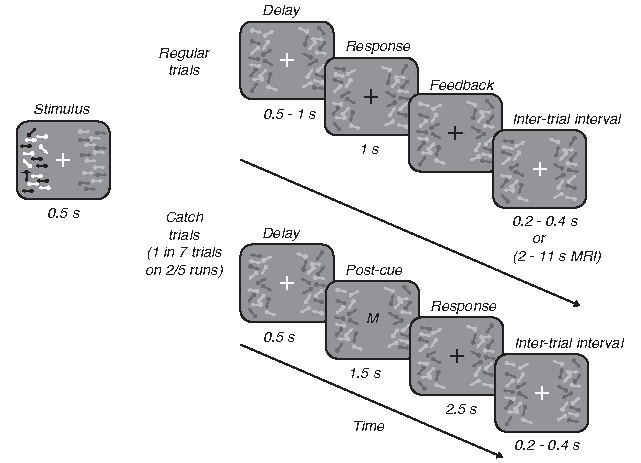
\includegraphics[keepaspectratio,width=0.5\textwidth]{figs_c2/Fig1_behav.pdf}
\caption[Behavioral task]{Behavioral task. Observers discriminated which of two random dot stimulus patches had higher contrast or coherence in different blocks of trials. Each block began with the word “contrast” or “motion” indicating that observers should report about contrast or coherence, respectively, and ignore the other feature. Between trials (Inter-trial interval) and during all but the Stimulus segment, the dot patches were presented at 25\% contrast with incoherent motion. On each trial both dot patches increased by independent base increments of contrast and coherence (+7.5, +15, +30, or +60\% contrast +15, +30, +45, or +60\% coherence) for 0.5s (Stimulus). In addition, for each feature one side was chosen independently to have an additional threshold-level increment, determined by a staircasing procedure. For regular trials, after a 0.5 - 1s period (Delay), observers were asked to report which side contained the additional increment in contrast or coherence (Response) and were given feedback (Feedback). On a subset (Catch trials) of runs (2/5) on rare trials (1/7) the delay period was followed by a post-cue (Post-cue), the letter “M” or “C”, indicating that the observers should prepare a response about the un-cued feature. Additional time was given to observers to make these decisions (post-cue period of 1.5 s, response window of 2.5 s) and observers did not receive feedback on catch trials.}
\label{fig:c4f1}
\end{figure}

We characterized human perceptual sensitivity to the contrast and coherence of moving dots while observers had to report exclusively about one feature and ignore the other. We measured observers’ just-noticeable differences (JND) in image contrast or motion coherence between a pair of simultaneously presented random dot stimulus patches in a two-alternative forced choice task (Fig \ref{fig:c4f1}). Each block of trials began with either the word ``contrast'', indicating that observers should report which dot patch had higher contrast while ignoring differences in coherence, or ``motion'', indicating the opposite. Each trial consisted of a 0.5 s base increment in the contrast and coherence of both dot patches (at all other times the dot patches were kept visible at 25\% contrast and 0\% coherence). In addition to this base increment a small additional increment near perceptual threshold was added to one side independently for each feature. Therefore, for every trial regardless of cueing condition there was a difference in both features between the two dot patches and each patch was equally likely to contain the additional increment. After stimulus presentation and a brief delay, observers reported which side had the higher magnitude of the cued feature and received feedback.

\subsection{Observers were able to report about each motion visibility feature independently.}

\begin{figure}
\centering
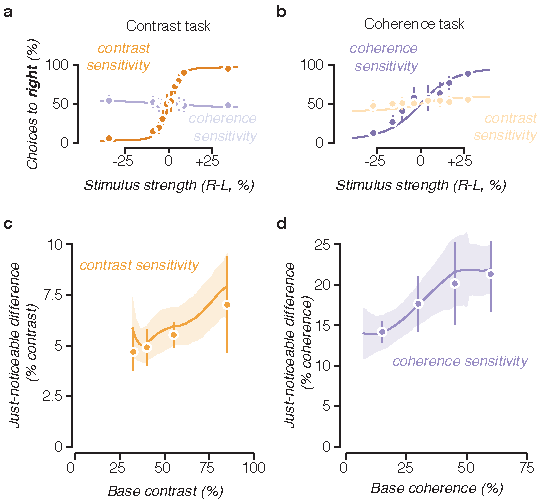
\includegraphics[keepaspectratio,width=0.5\textwidth]{figs_c2/Fig2_behav.pdf}
\caption[Perceptual sensitivity to contrast and motion coherence and fit of validation linking model]{Perceptual sensitivity to contrast and motion coherence and fit of validation linking model. (a) Contrast task. The markers plot the average probability across observers and base stimulus strengths of indicating that the right dot patch had higher contrast or motion coherence while performing the contrast task, as a function of the difference in contrast (orange) or coherence (blue) between the two patches. Curves plot the predictions of the eight-area linking model using measurements made during passive viewing. These were fit to each individual observer’s behavioral data with a flexible readout, therefore fitting each task separately. (b) Coherence task, conventions same as (a). (c) Markers plot the just-noticeable difference for contrast during that task estimated from a Weibull function fit for each base stimulus strength, averaged across observers. Curves indicate the average prediction of the 8-area linking model across observers. (d) Same as (c) for the coherence task. All markers indicate the mean and error bars the 95\% confidence interval across observers. Curves indicate the mean model prediction across observers and shaded areas the 95\% confidence intervals. Some error bars are hidden by the markers.}
\label{fig:c4f2}
\end{figure}

Collapsing across observers and base stimulus strengths we found that observers were sensitive to the feature they were asked to report (dark orange, Fig. \ref{fig:c4f2}a, and dark purple, Fig. \ref{fig:c4f2}b), but insensitive to the features they were asked to ignore (light purple and light orange, Fig. \ref{fig:c4f2}a and \ref{fig:c4f2}b). The psychometric functions (circle markers in Fig. \ref{fig:c4f2}a) were well fit by cumulative normal distributions (not shown, average cross-validated $r_{pseudo}^2=87.7$\%). This suggests that observers’ decisions were consistent with a signal detection process in which two sensory representations were compared subject to Gaussian noise. Separating out sensitivity by base stimulus strength, we observed a proportional increase in just-noticeable differences (Fig. \ref{fig:c4f2}c-d) reminiscent of Weber's law. Weber’s law states that the slope of this relationship should be 1 on a log-log axis but we found slopes less than one for contrast, 0.44, 95\% CI [0.41 0.50], consistent with previous studies (Gorea and Sagi, 2001; Pelli, 1985; Pestilli et al., 2011), and 0.81, 95\% CI [0.78 0.85] for coherence. Fitting a Weibull function on a subject-by-subject basis for base contrasts 32.5, 40, 55 and 85\% we found just-noticeable differences in contrast (Fig. 2c) to be 4.6\%, 95\% CI [3.8, 5.5], 4.8\%, 95\% CI [3.9, 5.8], 5.5\%, 95\% CI [4.9, 6.2], and 7.5\%, 95\% CI [5.3, 9.8], respectively. For base coherences 15, 30, 45, and 60\% we found just-noticeable differences in coherence (Fig. 2D) to be 14.2\%, 95\% CI [12.9, 15.5], 17.7\%, 95\% CI [14.3, 21.1], 20.2\%, 95\% CI [15.1, 25.3], and 21.3\%, 95\% CI [16.7, 25.9], respectively. Note that for contrast the base stimulus strengths are reported as the absolute value and not the relative increment from the 25\% contrast and incoherent motion that was shown continuously throughout the experiment.

\subsection{Changes in cortical representation of motion visibility during task performance}

\begin{figure}
\centering
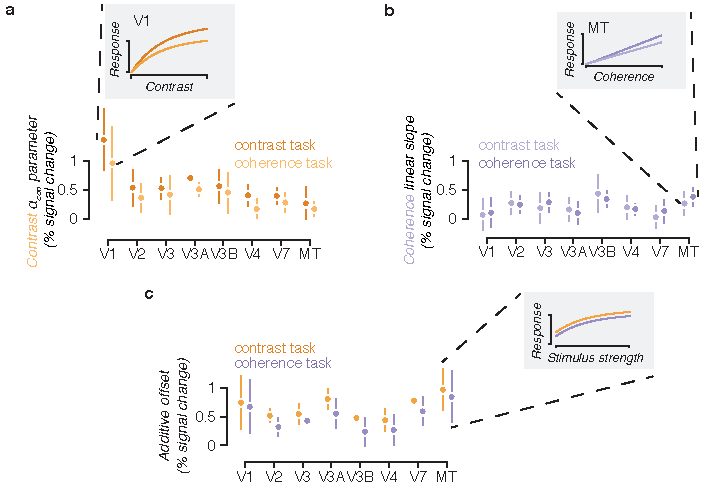
\includegraphics[keepaspectratio,width=0.5\textwidth]{figs_c2/Fig3_active.pdf}
\caption[Cortical measurements during active viewing]{Cortical measurements during active viewing. Observers performed the behavioral task while hemodynamic responses in retinotopic visual cortex were measured. (a) The average across observers of the $\alpha_{con}$ parameter, a measure of contrast sensitivity, is shown for each task context (dark and light markers are the contrast and coherence task, respectively). Inset shows how the change in the parameter affects the change in the contrast response function for V1, ignoring any change in additive offset. (b) As in (a) for coherence sensitivity as measured by the linear slope of the coherence response function (dark and light markers are coherence and contrast task, respectively) and inset shows the relationship for MT. (c) As in (a-b) for the $\alpha_{task}$ parameter which absorbs additive offsets. Inset shows the additive offset shift for MT.}
\label{fig:c4f3}
\end{figure}

We measured BOLD signal in retinotopically defined visual areas and found small changes in sensory responses when observers switched between reporting contrast and coherence (Fig. 3). Ten of the observers who performed the behavioral experiments repeated the task in the magnet. We used these measurements to examine how the contrast and coherence responses changed, either by multiplicative gain or additive offset, in each visual area (see Methods). For a majority of subjects, we found that when reporting about contrast, compared to reporting about coherence, the response to contrast in cortex showed a multiplicative gain (Fig. \ref{fig:c4f3}a). The average increase in $\alpha_{con}$ (Eq. \ref{eqn:c4conresp}) over areas and observers was 0.13\% signal change / unit contrast, 95\% CI [0.07, 0.19]. The direction of this effect wasn’t always consistent, in V1 8/10 observers showed an increase; for V2 6/10; V3 7/10; V4 7/10; V3a 7/10; V3b 7/10; V7 5/10; MT 6/10. For the coherence response, we found no consistent change in the slope of the response function when reporting about coherence \ref{fig:c4f3}b). The average over areas and observers was -0.02\% signal change / unit coherence, 95\% CI [-0.08, 0.04]), though some individual areas like MT showed an increase. These changes were inconsistent across observers, in V1 6/10 observers showed an increase in the linear slope of the coherence response; V2 6/10; V3 6/10; V4 6/10; V3a 4/10; V3b 5/10; V7 6/10; MT 6/10). In some linking models additive offsets have been shown to account for the perceptual benefits of selective attention \citep{Pestilli2011-gi}. We found that reporting about the stimuli, rather than passively viewing them, led to an additive offset in most visual areas (Fig. \ref{fig:c4f3}c). Average increase in $\alpha_{task}$ (Eq. \ref{eqn:c4Rarea}) over areas and observers compared to passive viewing was 0.36\% signal change, 95\% CI [0.30, 0.44]. Additive offsets were slightly larger during the contrast task than the coherence task (Fig. \ref{fig:c4f3}c). Averaged over areas and observers this effect was a modest 0.07\% signal change, 95\% CI [0.01, 0.14]. In summary, we measured small changes in sensory response between task conditions and found that in some cortical areas contrast sensitivity increases when subjects perform the contrast task and coherence sensitivity increases when subjects perform the coherence task. While these changes are in the right direction to underlie task performance, a formal linking model is required to determine if they are large enough to account for perceptual behavior.

\subsection{Linking model between cortical representation and perception of motion visibility}

\begin{figure}
\centering
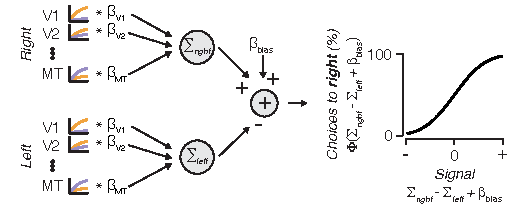
\includegraphics[keepaspectratio,width=0.5\textwidth]{figs_c2/Fig4_linkingmodel.pdf}
\caption[Readout linking model]{Readout linking model. The linking model simulates the cortical response evoked by each dot patch according to an existing framework (Birman and Gardner, 2018) which parameterized the contrast response function (orange curves) as a Naka-Rushton and the coherence response function (blue curves) as linear, or a saturating exponential function. The model weights the cortical responses from each visual area ( values) evoked by the stimulus (Right or Left) according to the current task. The model then takes the difference between the signals evoked by each stimulus, plus a bias term (bias) to account for any individual observer’s bias to choose one response over the other. To convert from this weighted signal to probability of choosing the patch on the right, the signal is passed through a cumulative normal distribution (curve on right). The linking model is analogous to probit regression with nonlinear input signals.}
\label{fig:c4f4}
\end{figure}

We set out to build such a linking model (Fig. 4) that could quantitatively predict behavioral performance from measurements of cortical sensory representation. Once validated, such a model could then be used to assess whether the sensory changes we measured were large enough to explain behavioral performance in the task conditions. Linking models have been built for contrast discrimination tasks by assuming that higher contrast is detected by comparing the magnitude of cortical responses evoked by different stimuli, subject to some noise (Boynton et al., 1999; Foley and Legge, 1981; Gardner, 2015; Ling and Carrasco, 2006; Nachmias and Sansbury, 1974; Pestilli et al., 2009). Behavioral sensitivity is determined by the ratio of response difference to the standard deviation of the noise, as in the classic signal detection measure d’. In our task, cortical responses are the result of stimuli that differ both in contrast and coherence. The linking model therefore needed to be able to differentiate which feature caused a difference in response. We reasoned that this could be accomplished by properly weighting visual areas with different sensitivity to each stimulus feature. Our model took the form of a probit regression (Bliss, 1934) in which the difference in weighted response of visual areas to the two stimuli were computed and passed through the cumulative normal distribution to predict the probability of different choices (Fig 4, see Methods: Linking model for full description).

Before evaluating such a model on the measurements of cortical activity during task performance (Fig. 3), we wanted to validate that such a linking model could in principle account for contrast and coherence discrimination. In previous work we published measurements of contrast and coherence response in cortex while observers passively viewed the same random dot stimuli used here (Birman and Gardner, 2018). These measurements were used to quantify the shape of contrast and coherence responses across retinotopically defined visual areas using functional forms (Naka-Rushton for contrast and a saturating exponential form for coherence, see Eq. 4 and 5). These passive-response data showed, for example, that V1-V4 are relatively more sensitive to changes in image contrast, whereas MT is more sensitive to changes in motion coherence. For reference, the parameters describing these differences in sensitivity are reported in the Methods (for additional details see: Birman and Gardner, 2018). Using the functional forms measured during passive viewing we simulated the trial-by-trial response of eight visual cortical areas, V1-V3, V4 (hV4), V3A, V3B, V7, and MT (hMT+), and modeled sensory readout on each trial as a task-dependent linear weighting of the population responses (Fig. 4). This resulted in a scalar response for the left and right stimulus patches (Σ_right, Σ_left) on each trial. The observer’s decision about which side had the higher cued feature was modeled as a comparison between these two scalar responses (Σ_right-Σ_left) summed with a side bias (β_bias). This scalar decision variable was subject to Gaussian noise as implied by the cumulative normal of the probit link function. We fit the parameters of the linking model using maximum likelihood estimation for each observer (8 cortical area weights x 2 task conditions + 1 bias parameter = 17 total parameters) using the average population response functions from Birman & Gardner (2018). 

We found that the linking model based on the passive viewing BOLD data was a good fit for the behavioral measurements (curves, Fig. 2), capturing both the shape of the psychometric functions and the increase in just-noticeable differences with increasing base stimulus strength. To evaluate models we examined Tjur’s coefficient of determination (CD), a measure intended to be interpreted similarly to r^2 for models of binary decisions (Tjur, 2009). To compare models, we computed cross-validated log-likelihood ratios (see Methods: Model comparison). We found across observers an average CD of 0.44, 95\% CI [0.42, 0.45] reflecting that the model captured the sensitivity of human observers to differences in visibility across both task conditions (curves, Fig. 2a-b) as well as the reduced sensitivity at increasing base stimulus strength (curves, Fig. 2c-d). The fits shown are for the 8-area model, but we also tested a model with only the two areas with the highest contrast and coherence sensitivity, V1 and MT (2 cortical area weights x 2 task conditions + 1 bias parameter = 5 total parameters). We found a similarly good fit, log⁡(L_2/L_8 )= 7.38, 95\% CI [-3.09, 32.78]. The average CD of the 2-area model was also 0.44, 95\% CI [0.43, 0.45].

\begin{figure}
\centering
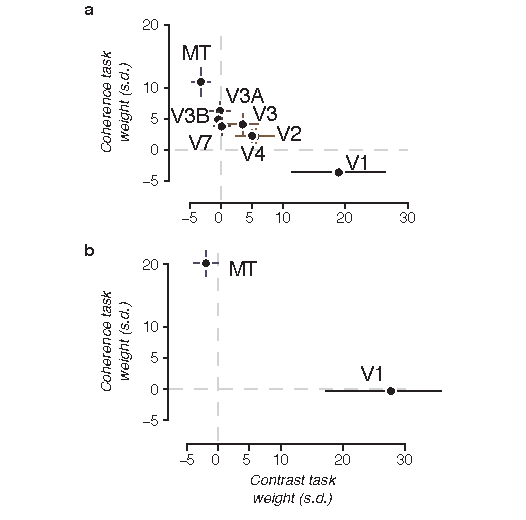
\includegraphics[keepaspectratio,width=0.5\textwidth]{figs_c2/Fig5_weights.pdf}
\caption[Cortical area weights]{Cortical area weights. (a) The weights of the flexible-readout model fit to passive viewing data are shown for the contrast task (x-axis) and coherence task (y-axis) for the eight cortical areas we defined retinotopically: V1, V2, V3, V4 (hV4), V3A, V3B, V7, and MT (hMT+). (b) As in (a) but for the 2-area model with only V1 and MT. All markers indicate the mean across observers and error bars the 95\% confidence intervals.}
\label{fig:c4f5}
\end{figure}

The linking model fit weights according to the relative sensitivity of each cortical area to contrast and coherence (Fig. 5). In the 8-area model the contrast task weights (x-axis, Fig. 5a) are proportional to how sensitive each area is to contrast relative to coherence: V1-V4 have positive weights, while only MT was given a negative weight. The negative weight on MT counteracts sensitivity to coherence in V1-V4 and ensures the linking model was insensitive to coherence when reading out contrast. The weights for the coherence task (y-axis, Fig.5a) behaved similarly, with MT getting the largest positive weight and V1 a slight negative one. A similar pattern was observed for a model with only areas V1 and MT (Fig. 5b) but with less negative weighting in the coherence readout.  

\begin{figure}
\centering
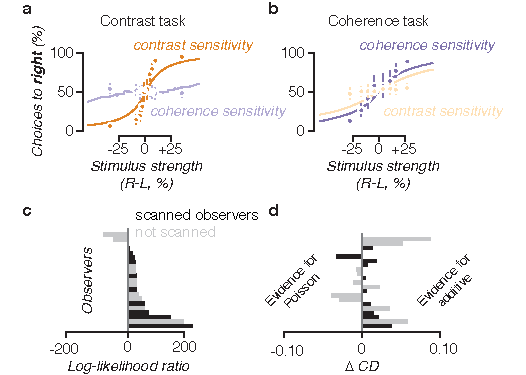
\includegraphics[keepaspectratio,width=0.5\textwidth]{figs_c2/Fig6_poisson.pdf}
\caption[Poisson vs. additive noise]{Poisson vs. additive noise. (a,b) Same conventions as Fig 2a and b, except curves indicate the prediction of a model incorporating Poisson-like noise in which variance scales equal to response strength. (c) The cross-validated likelihood ratio (difference in log-likelihood) between the additive and Poisson models is shown for each observer. (d) The change in Tjur’s CD comparing the additive models against the Poisson models, a measure analogous to $r^2$. Observers are sorted as in (c). In panels (c) and (d) evidence for the Poisson model is plotted towards the left and evidence for the additive model to the right.}
\label{fig:c4f6}
\end{figure}

Using model comparison, we validated our linking model assumptions that noise is additive and that observers had no dependency on choice history. Models based on single-unit variability often assume a Poisson-like noise (Softky and Koch, 1993), but because our model is based on population activity for which independent single-unit variable would be expected to average out, we modeled an additive noise component. This choice of additive Gaussian noise was important. A model using Poisson noise which increased with stimulus strength did not fit the data (Fig. 6). On average across observers the additive model was a better fit compared to the Poisson model, $\log(\frac{\mathcal{L}_{additive}}{\matchcal{L}_{Poisson}})$)= 43.58, 95\% CI [18.84, 77.93] (Fig. 6c) and improved CD by 0.01, 95\% CI [0.00, 0.02] (Fig. 6d). A number of studies have found that observers performing psychophysical tasks are biased by previous choices even when those choices are uninformative for the current trial \citep{Abrahamyan2016-od} (Frund et al., 2014). We also tested for possible biases due to choice history (see Methods) but found that including these additional fit parameters caused the cross-validated log-likelihood to deteriorate, suggesting over-fitting, $\log(\frac{\mathcal{L}_{original}}{\matchcal{L}_{stay/switch}})$= 3.66, 95\% CI [0.31, 9.08]. Thus, model comparison was able to validate that choice history effects were negligible, and that noise was best assumed to be additive rather than Poisson.

\subsection{Using the linking model to test fixed vs flexible readout}

\begin{figure}
\centering
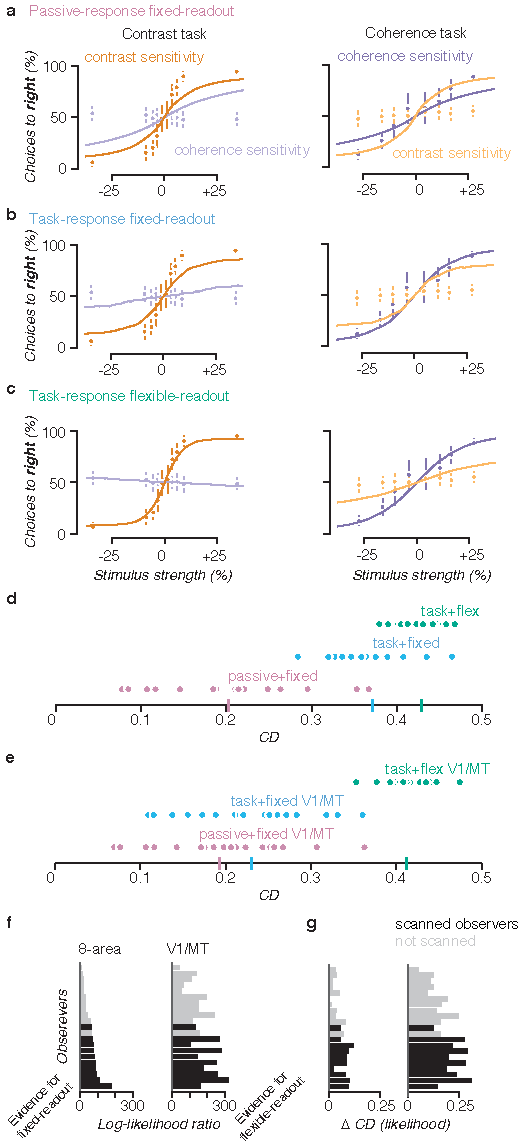
\includegraphics[keepaspectratio,width=0.5\textwidth]{figs_c2/Fig7_readout.pdf}
\caption[Comparing fixed- and flexible-readout linking models]{Comparing fixed- and flexible-readout linking models. (a-c) Same conventions as Fig. 2a and b, except curves plot: (a) the fit of the passive BOLD measurements with a fixed readout, (b) the BOLD measurements during task performance with a fixed readout, and (c) the BOLD measurements during task performance with a flexible readout. The fixed-readout model forces any change in perceptual sensitivity to be the result of differences in sensory response between tasks by using only a single set of cortical readout weights (eight weights and one bias term). The flexible-readout model allows a different set of weights for each task condition (sixteen weights and one bias term). (d) Tjur’s $CD$ for the models in (a-c). Averages are shown as a bar on the axis. (e) Conventions as in (d) for the 2-area models with only V1 and MT. (f) Model comparison of the cross-validated likelihood ratio (difference in log-likelihood) between the task-response fixed-readout and task-response flexible-readout models. Evidence for the fixed-readout model is plotted to the left and flexible-readout to the right (none of the fits are in favor of the fixed readout model) (g) As in (f) for Tjur’s $CD$. Markers in panels a-c indicate the average across observers. Markers in panels d and e indicate individual observers. Error bars are the 95\% confidence intervals. Some error bars are hidden by the markers.}
\label{fig:c4f7}
\end{figure}

Having verified the linking model based on passive viewing data, we now asked whether the small changes in sensory representation which we measured during task performance could account for how perceptual sensitivity changed when observers switched task. If sensory changes were sufficiently large, then the readout could be fixed between task conditions. Such a fixed readout model would only require a single set of cortical area weights with changes in perception accounted for only by changes in sensory responses. 
As a baseline for comparison, we first fit the fixed-readout model on the sensory responses measured during passive viewing where by definition there are no sensory changes between task conditions. This passive-response fixed-readout model can only produce behavior that is intermediate between the two tasks. That is, it is sensitive to both contrast and coherence (Fig \ref{fig:c4f7}a, orange/yellow contrast curves and blue/purple coherence curves are not flat) and cannot switch sensitivity between the two tasks (Fig \ref{fig:c4f7}a, curves for left and right panels are identical).  The CD and likelihood of the passive-response fixed-readout model provide a lower bound on the possible explainable variance (Fig. \ref{fig:c4f7}d and e). 

Fitting the fixed-readout model to sensory responses measured during task performance showed that while changes in sensory response could account for a substantial amount of the behavioral performance, the changes were insufficiently large to fully explain task performance. This task-response fixed-readout model achieved a better fit of the behavioral data than the passive-response fixed-readout model (Fig. 7d and e, compare magenta and blue points) thus quantifying how much the sensory changes reported above can account for behavioral performance. Indeed, the task-response fixed-readout model was better able to capture differences in behavior between the contrast and coherence task (Fig 7b, compare curves for left and right columns). However, the linking model failed to completely capture the ability of subjects to change their perceptual sensitivity to contrast and coherence between the two tasks. In the contrast task, the contrast sensitivity curve (orange, Fig 7b) does not match the sensitivity of the observers and the model predicted a weak bias for coherence (light purple, left panel Fig 7b) that the subjects did not show. In the coherence task, the coherence performance was reasonably well-matched (purple curve, right panel), but the model predicted strong bias from contrast (orange curve).

Rather than rely only on changes in sensory representation between tasks, a linking model that could read out responses from visual areas differently between tasks was better able to fit the behavioral performance. We tested this task-response flexible-readout model by allowing the weights for different visual areas to change between tasks while still using the sensory responses measured during task performance. This model provided reasonable fits to the behavioral data (Fig. \ref{fig:c4f7}c), capturing the performance during the contrast task (left column), although it did predict more bias to contrast during the coherence task then the observers displayed (orange curve, right panel). Because the fixed-readout and flexible-readout models had different numbers of parameters (fixed-readout = 9 parameters, flexible-readout = 17) it was critical to evaluate the models with a cross-validated metric. We found that for the task-response measurements the flexible-readout model was a far better fit than the fixed-readout model (Fig. 6f and g), log⁡(L_Flexible/L_Fixed )= 60.16, 95\% CI [44.90, 77.75], difference in CD, 0.06, 95\% CI [0.04, 0.07]. Note that observers who we measured physiology for (black bars, Fig. \ref{fig:c4f7}f and g) show a larger improvement in model fit compared to the other observers, which we attribute to an effect of increased training.

Observers who we measured physiology for (black bars, Fig. 6C and D) show a larger improvement in model fit compared to the other observers (gray bars). One explanation for this effect is that the observers we measured in the scanner were better able to ignore the irrelevant feature due to having more practice. The fixed readout model, which predicts an inability to ignore the irrelevant feature, would then fail more dramatically for better-trained observers. Indeed, observers who were a part of the scanning were slightly better (n=11 observers, mean just-noticeable difference for contrast 5.62\%, 95\% CI [4.98, 6.50], and coherence 18.06\%, 95\% CI [16.32, 21.15]) compared to observers who did not participate in scanning (n=10, mean just-noticeable difference for contrast 10.02, 95\% CI [6.23, 19.95], and coherence 21.40\%, 95\% CI [18.64, 25.03]). 

As additive offsets have been used with a fixed readout to explain behavioral performance differences with spatial attention \citep{Pestilli2011-gi}, we also tested an efficient selection model that weights responses according to their magnitude, but found that this model also could not explain the behavioral performance. An increase in additive offset during one task condition or the other could be used by an efficient selection model that weighs signals by their magnitude \citep{Hara2014-mv,Pestilli2011-gi}, e.g. selecting out V1 during the contrast task and MT during the coherence task. On average response magnitudes did increase a moderate amount when observers performed the task compared to the passive viewing condition, but these additive offsets were similar for both tasks (Fig. \ref{fig:c4f5}C). We found that the flexible model was a far better explanation than an efficient selection model (see Methods for implementation details), log⁡(L_Flexible/L_Selection )= 130.39, 95\% CI [109.66, 151.31], difference in CD, 0.30, 95\% CI [0.28, 0.32]. 

\subsection{Behavioral evidence for a flexible readout}

One advantage to keeping sensory representations relatively stable is that observers can maintain information about unattended features. To measure whether observers could recall unattended information we included ‘catch’ trials in the behavioral task. In catch trials, observers were shown a post-cue after stimulus presentation which indicated that they should report about the un-cued feature (bottom time line, Fig. \ref{fig:c4f1}). Observers made these reports despite the stimulus having already been presented and despite having already had 0.5 s to prepare their response for the main task. We were able to ensure observers did not split their attention by keeping the main task at perceptual threshold, making catch trials rare, and not providing feedback.

Because observers were told at the start of each block (~65 trials or 4 minutes) whether or not catch trials would occur there is a concern that they could have split their attention, but we found no evidence for this. In other dual task settings there is a significant cost associated with performing two tasks at the same time (Sperling and Melchner, 1978), especially when one or both tasks are difficult (near perceptual threshold). Note that we designed the catch trials to minimize this effect by making them rare and not providing feedback. If observers split their attention, we would expect to detect an increased just-noticeable difference (JND) on the cued main task. Instead, we found that the just-noticeable differences were similar: on runs with catch trials the contrast task JND increased by only 0.19\% contrast, 95\% CI [-0.19, 0.78], and for the coherence task by 0.74\% coherence, 95\% CI [-0.76, 3.13].  

During catch trials we found that observers were less sensitive to the un-cued motion visibility features compared to when they were cued, but nevertheless they maintained significant information about the unattended features. Observers’ just-noticeable differences were larger on the catch trials both for the contrast task (average $\Delta$ just-noticeable difference = +5.30\% contrast, 95\% CI [+3.83, +7.22]) and coherence task ($\Delta$ just-noticeable difference = +45.84\%, 95\% CI [+26.17, +98.23]) (Fig. 7). These averages (and subsequent analysis) exclude 4/21 and 1/21 observers for the coherence and contrast tasks, respectively, because they could not perform the task and their just-noticeable differences were not measurable (i.e. their JND was more than what could be displayed on the screen). 

\begin{figure}
\centering
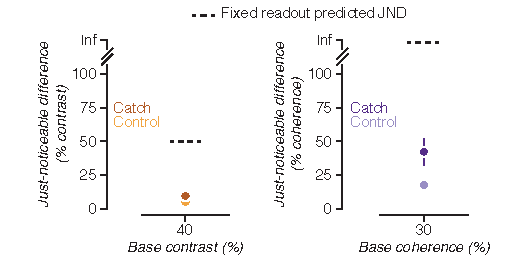
\includegraphics[keepaspectratio,width=0.5\textwidth]{figs_c2/Fig8_catch.pdf}
\caption[Perceptual sensitivity on catch trials]{Perceptual sensitivity on catch trials. Just-noticeable differences (JND) for contrast (left) and coherence (right) are shown for the regular (control, light colors) and catch (dark colors) trials during runs that included catch trials. Predicted just-noticeable differences for catch trials are shown for the fixed readout model (dashed lines). Markers indicate the average across observers and error bars the 95\% confidence intervals, some error bars are hidden by the markers. }
\label{fig:c4f8}
\end{figure}

If observers had a fixed readout which could not switch to the ignored feature during catch trials, then they would be forced to use the wrong readout and performance would be extremely poor. We found that this fixed readout model predicted much higher just-noticeable differences than measured and therefore could not account for catch trial behavior. That is, we used the task-response flexible-readout model to compute the expected JND on catch-trials assuming that observers were unable to switch the readout to the post-cued feature. For example, for the contrast-task in which the catch trials required making a coherence judgement, we used the cortical readout weights for the contrast-task ($\beta_{V1}$,$\beta_{V2}$,...), and vice-versa. This model underestimated human performance on catch trials (dashed lines, Fig. \ref{fig:c4f8}). On contrast catch trials (i.e. post-cued trials when observers reported about contrast, during a run where the main task was coherence) the model predicted just-noticeable differences of 56.9\%, 95\% CI [33.8, 80.1], but the average observer had a JND of only 10.1\% contrast, 95\% CI [7.5, 12.7]. On coherence catch trials the model predicted that observers would be incapable of performing the task but the average observer JND was 40.8\% coherence, 95\% CI [32.4, 49.2]. 

Instead, we found that a better explanation for catch trial behavior came from a readout which could dynamically change within trials but incurred an additional cost for maintaining sensory information in working memory. This cost could be due to a drop in the signal-to-noise of the sensory representation, perhaps due to responses degrading over time. We estimated the cost by dividing the thresholds measured during catch trials by the thresholds measured during regular trials. This approach suggests that on average σ increased (or responses degraded) for coherence by a factor of 3.44, 95\% CI [2.46, 5.90] and for contrast by 2.21, 95\% CI [1.87, 2.66]. The overlap in estimates suggests a single cost, i.e. the change from a discrimination task to a working memory task, might govern the change in performance for both tasks; averaging the increase in noise gives an estimated reduction in sensitivity of 2.83, 95\% CI [2.31, 4.17]. Thus, a model which allows rapid re-weighting, combined with a fixed cost for using working memory, can explain behavioral performance for both contrast and coherence catch trials.

\section{Discussion}

We found that observers were able to independently judge the visibility of patches of moving dots based on either their contrast or coherence. Concurrent measurements of BOLD activity showed that there were small changes in sensory representations during task performance. Cortical responses were somewhat more sensitive to contrast during contrast discrimination and, in some areas like MT, more sensitive to coherence during the coherence task. Our analysis with a fixed-readout linking model showed that these changes could account for some, but not all of the behavioral performance. Instead, the behavior was consistent with a flexible readout of sensory representations. Keeping representations relatively stable should allow observers to retain information about unattended features and we found that during catch-trials this was the case. Our results highlight the importance of using models that quantify the link between cortical representation and perception.

\subsection{Linking models for human motion visibility perception}

We manipulated the contrast and coherence of random dot motion stimuli because of the extensive existing knowledge of how neural representations of these features are related to  visual perception (Gold and Shadlen, 2007) and because their similar representation in cortex suggests that changing the representation of one will necessarily affect the other. Contrast, the average difference between bright and dark \citep{Bex2002-it}, and coherence, the percentage of dots moving in the same direction, both control the visibility of motion. Human cortical visual areas are known to be sensitive to these properties such that an increase in visibility results in monotonically increasing responses throughout visual cortex \citep{Avidan2002-jg,Birman2018-sp,Britten1993-oh,Gardner2005-pg,Logothetis2001-kk,Olman2004-dd,Boynton1996-ff,Olman2004-dd,Rees2000-ul,Tootell1998-bb}(Simoncelli and Heeger, 1998). For observers to judge these two features independently their sensory representations need to be separated according to context, a step which existing linking models built for single features have not had to contend with.

The computational steps from sensory representation to perception have been well characterized for contrast discrimination. In these linking models an observer’s choice is computed by comparing the evoked neuronal responses to different stimuli (Boynton et al., 1999; Foley and Legge, 1981; Ling and Carrasco, 2006; Nachmias and Sansbury, 1974; Pestilli et al., 2009). Individual neurons exhibit monotonically increasing responses to contrast \citep{Albrecht1982-rq}, with different parameterizations \citep{Tolhurst1983-cv} that can be pooled into a population response \citep{Shadlen1996-pr}. Such population responses to contrast are well-indexed by BOLD signal in human visual cortex \citep{Avidan2002-jg,Boynton1996-ff,Boynton1999-jd,Gardner2005-pg,Heeger2000-pq,Logothetis2001-kk}. Linking models have been shown to account for BOLD signal measurements and perceptual responses during contrast discrimination tasks \citep{Boynton1999-jd}, predict changes in these measures during surround masking \citep{Zenger-Landolt2003-kq} and detection \citep{Ress2000-pa}, and have been used to describe the selection of signals from attended locations \citep{Hara2014-mv,Pestilli2011-gi}. 

Our model extends a linking model of contrast discrimination \citep{Boynton1999-jd} to simultaneous judgments of contrast and coherence. To separate the intertwined sensory representations of these features we allowed a linear weighting of cortical areas. The weights fit by the model confirmed that the bulk of information for these simple perceptual decisions was available in V1 for contrast perception and MT for coherence. This matches with previous results implicating monkey MT in judgments about motion \citep{Britten1996-ik,Katz2016-xc,Newsome1988-os}. But the weights also revealed that other areas could play an important role in perception by suppressing correlated signals about un-cued features in the readout. Our linking model is also specific to the random dot stimulus we chose. Changing the dot density (Smith et al., 2006) or aperture size \citep{Ajina2015-xm,Becker2008-uj,Costagli2014-kg} can result in decrements or zero response to increasing coherence, which would necessitate a linking model specific to those stimulus properties. We chose our stimulus size, dot density, and dot speed with these concerns in mind (for additional discussion of how stimulus properties affect the coherence response see Birman and Gardner, 2018).  

The linking model we developed held only if sensory noise was modeled as additive but not if variability increased in proportion with firing rate \citep{Softky1993-ki}. Additive noise appears repeatedly in the literature using linking models (Boynton et al., 1999; Hara and Gardner, 2014; Pestilli et al., 2011; Sapir et al., 2005), in purely psychophysical approaches (Gorea and Sagi, 2001; Neri, 2018, 2010), and in measurements of population activity from voltage sensitive dyes (Chen et al., 2006). In our results, the Poisson noise model failed because it combined increasing noise with response functions that saturate \citep{Birman2018-sp}; either of which alone predicts the cumulative normal form of the psychometric functions and a Weber-law like effect at increasing base stimulus strengths. This result suggests that the noise that limits perceptual behavior is not the individual variability in firing rate of single neurons, which presumably is averaged out across a population, but a correlated source of variability which is not dependent on response amplitude.

\subsection{Flexible readout of sensory representations}

Our results demonstrate that sensory change due to attention does not transform the sensory representation directly into a form that can be used to drive motor responses. Instead, switching from reporting one stimulus property to another must change the readout (i.e. weighting of connections), which may begin to occur in sensory cortices (Ruff and Cohen, 2017) but must also extend beyond them. One possible role for the response gain is that it works together with changes in readout, acting, as we calculated, as a weak form of sensory enhancement. Recent theoretical and experimental results suggest that such changes might improve the ability of a linear readout to differentiate between stimulus-driven and internal signals \citep{Ecker2016-ro,Rabinowitz2015-uz,Snyder2018-yr}. These changes match with our finding that noise limiting perceptual sensitivity is due to correlated internal variability. Sensory changes might also drive responses to be more aligned with the readout dimension (Ruff and Cohen, 2019), effectively working together.  

Although for our task the scale of sensory changes provided only a partial explanation for context-dependent behavioral reports, this need not always be the case. In the literature on visual attention there are many examples of changes in sensory representation as a result of task demands \citep{Carrasco2011-xp}. We interpret these results and our own as falling within a continuum where task demands are implemented by complementary changes in sensory representation and sensory readout. Sensory effects that can alone account for behavioral changes would be at one end of this continuum. For example, measurements of changes in spatial tuning \citep{Kay2015-pd,Klein2014-oe,Vo2017-oi} may underlie bottom-up biases in spatial perception \citep{Klein2016-ox}, additive shifts in response \citep{Buracas2007-pe}( Li et al., 2008; Murray, 2008) can be used by efficient selection mechanisms (Chen and Seidemann, 2012; Hara and Gardner, 2014; Pestilli et al., 2011) to account for perceptual threshold enhancement, and changes in correlation structure during focal spatial attention (Mitchell et al., 2009) can be sufficient to explain changes in perceptual sensitivity (Cohen and Maunsell, 2010, 2009; Ruff and Cohen, 2019). These spatial attentional effects may reflect the combination of a fixed sensory readout combined with changes in representation which select \citep{Carrasco2011-xp} and align \citep{Ruff2018-yx} relevant signals while suppressing others.

Our results suggest that judgments of motion visibility rely on both a context-dependent readout and changes in sensory representation, putting our task in a different part of the continuum described above. Relying on flexible readout could help maintain adaptability in the face of uncertain task demands. It is possible that given enough time and task-consistency observers could have shifted their cortical implementation to solve our task using a fixed readout. This could be done by learning to pre-select relevant sensory representations, saving computational cost and speeding decision making. Similarly, sensory representations may be kept stable for visual features that are relevant for a variety of behaviors. For example, scene gist is known to survive inattention, both perceptually \citep{Li2002-ji} and as information that can be decoded from BOLD signal measurements of visual cortex \citep{Peelen2009-us}. 
How the human brain implements task demands may depend not only on the form of sensory representation, the precise task demands, and the extent of learning, but also on the associated computational costs \citep{Gardner2019-ky}. Flexible readout might be implemented by parts of prefrontal cortex which re-represent visual information in a context-dependent manner \citep{Bugatus2017-wl}, using dynamical properties that can selectively integrate different features of sensory stimuli \citep{Mante2013-tn}. Engaging these mechanisms requires resources to represent and process aspects of sensory stimuli that may not be behaviorally relevant. Changing sensory representations and using a fixed readout may instead reflect a computationally efficient solution where the visual system no longer has to contend with representing irrelevant stimulus information. In general, the complimentary mechanics of sensory change and change in readout are both essential tools for the human brain, allowing us to meet the demands imposed by daily life where constant shifts in attention are necessary to achieve our goals.

\chapter[Discussion]{Discussion and future directions}

\section{Summary and significance of findings}

\section{Directions for future investigations}


...
\appendix
...

\bibliographystyle{plain}
\bibliography{library}
\printbibliography



\end{document}